\documentclass[../main]{subfiles}
\begin{document}

% Indentation and spacing
\preto\subsection{\FloatBarrier}
\preto\section{\FloatBarrier}

\chapter{Multi-Frequency Simulations}

In this chapter, multi-frequency simulation campaigns are performed to answer the questions discussed 
in the first chapter: whether the number of superpositions affects the accuracy of the multi-frequency 
method, if so how many superpositions are appropriate in the multi-frequency method and which parameter 
limits that number, and where the source of error in the multi-frequency method lies, if it exists.

First, simulation parameters for the multi-frequency analysis are defined based on 
the results obtained from the signal analysis and nonlinearity studies. 
These parameters are then applied to two sets of multi-frequency campaigns, and the results 
are compared with the single-frequency analysis. 
Finally, a framework is formulated for the selection of frequencies and amplitudes for the multi-frequency analysis. 
This chapter is organised as follows:

\begin{flushleft}
\hspace{2cm}1. Simulation Parameters \\
\hspace{2cm}2. Multi-Frequency Analysis - 1 \\
\hspace{2cm}3. Multi-Frequency Analysis - 2 \\
\hspace{2cm}4. Framework for Multi-Frequency Analysis \\
\end{flushleft}

% ============================================================
\section{Simulation Parameters}
% ============================================================

The following criteria govern the selection of frequencies and amplitudes for the 
multi-frequency analysis:

\begin{enumerate}
    \setlength{\itemsep}{0pt}\setlength{\parskip}{0pt}
    \item Frequencies must lie within a frequency bin, as derived from the signal analysis.
    \item Prescribed motion amplitudes must be less than the threshold amplitude for nonlinearity, as derived from the nonlinearity study.
\end{enumerate}

All other simulation parameters are kept the same.\\

Based on these criteria, two sets of multi-frequency campaigns are performed. For both simulation 
campaigns, the frequency superpositions are kept identical, but the prescribed motion amplitude is differed. 
In the first campaign, the sum of the heave and pitch motion amplitudes for each 
superposition is kept below the nonlinearity threshold.
In the second campaign, the individual heave and pitch amplitudes are kept below the 
threshold. Since the frequency selection is the same for 
both campaigns, the frequency superpositions are described once in this section, while the 
amplitude selections are described in their corresponding analysis sections.\\

% ------------------------------------------------------------
\subsection{Selection of Frequencies and Superpositions}
\label{sec:Selection of Frequencies and Superpositions}
% ------------------------------------------------------------

To evaluate whether increasing the number of combined frequencies affects 
the accuracy of flutter derivative identification, eight frequencies are selected and 
organised into four superposition schemes. Superposition scheme~1 consists of single-frequency 
simulations and serves as the reference case. In Superpositions schemes ~2, 3, and~4, these 
frequencies are grouped into subsets of two, three, and four superpositions respectively
. The frequency selection procedure and the resulting superpositions 
are described below.\\

Within each superposition scheme, 
the lowest frequency (corresponding to the highest reduced velocity) is 
chosen first, with all other frequencies in the scheme selected relative to it. The lowest frequency may be 
chosen independently, but one important condition must be satisfied: its frequency bin spacing 
must be a definite number, so that the dependent frequencies fall exactly on the frequency bins.\\

For both campaigns in this study, the lowest frequency is set to $0.125$~Hz ( 
giving a corresponding reduced wind speed of $21.86$).\\

Allowing for 10 oscillations, the total simulation time is:
\begin{equation}
    t_{\text{total}} = \frac{1}{0.125} \times 10 = 80 \text{ s}
\end{equation}

With a time step size of $\Delta t = 0.002$~s, the total number of time steps is $40{,}000$.

The frequency bin spacing for a simulation with stable time of 80 seconds is,
\begin{equation}
    \Delta f = \frac{1/\Delta t}{N} = \frac{500}{40000} = 0.0125 \text{ Hz}
\end{equation}

Hence the frequency bins are $[0.0125,\ 0.0250,\ 0.0375,\ 0.0500,\ \ldots]$.\\

\textbf{Note:} The frequency spacing and frequency bins depend on the number of time steps. Therefore, if the simulation 
is interrupted, aerodynamic force and moment cannot be extracted accurately, as the frequency bins and 
spacing will be altered.\\

Dependent frequencies in the scheme are selected from the frequency bin list. An additional recommendation is to avoid selecting 
two frequencies that are adjacent within the frequency bin list. If one frequency does not 
align with a bin due to a shorter simulation duration, the result at the 
neighbouring frequency may also be corrupted through spectral leakage. To minimise this risk, 
sufficient spacing between selected frequencies is suggested.\\

The frequencies selected for simulation are shown in Table~\ref{tab:frequencies}. 
Frequencies are selected such that each frequency can serve as the primary frequency, 
providing flexibility in the superposition schemes. The frequencies $0.15$~Hz and $0.25$~Hz are exceptions, 
as they are also needed to cover the reduced velocity range for accurate interpolation of the 
flutter derivative curve.\\

\begin{table}[htbp]
\centering
\caption{Frequency Parameters for Multi-Frequency Analysis}
\label{tab:frequencies}
\begin{tabular}{|l|cccccccc|}
\hline
\textbf{Frequency (Hz)} & 0.125 & 0.15 & 0.2 & 0.25 & 0.4 & 0.8 & 1.6 & 3.2 \\
\hline
Reduced Velocity        & 21.86 & 18.21 & 13.66 & 10.93 & 6.83 & 3.42 & 1.71 & 0.85 \\
Stable Time Period (s)  & 80    & 80    & 50    & 40    & 25   & 12.5 & 6.25 & 3.125 \\
\bottomrule
\end{tabular}
\end{table}

% \textbf{Note:} The amplitude is identical for all frequencies; therefore, within each superposition, 
% only the frequencies are listed and may be matched against the table above.

The schemes are structured as follows.

\begin{itemize}
    \item \textbf{Superposition scheme 1:} Single frequencies (reference)

    \item \textbf{Superposition scheme 2:}
    \begin{itemize}
        \item $[0.125,\ 0.15]$
        \item $[0.2,\ 0.25]$
        \item $[0.4,\ 0.8]$
        \item $[1.6,\ 3.2]$
    \end{itemize}

    \item \textbf{Superposition scheme 3:}
    \begin{itemize}
        \item $[0.125,\ 0.15,\ 0.2]$
        \item $[0.25,\ 0.4,\ 0.8]$
        \item $[0.8,\ 1.6,\ 3.2]$
    \end{itemize}

    \item \textbf{Superposition scheme 4:}
    \begin{itemize}
        \item $[0.125,\ 0.15,\ 0.2,\ 0.25]$
        \item $[0.4,\ 0.8,\ 1.6,\ 3.2]$
    \end{itemize}
\end{itemize}

% ============================================================
\section{Multi-Frequency Analysis - 1}
% ============================================================

In this section, the sum of the heave and pitch motion amplitudes for each 
superposition is kept below the linearity limit value obtained from the nonlinearity study.

This section is organised as follows:

\begin{flushleft}
\hspace{2cm}1. Superposition Schemes \\
\hspace{2cm}2. Procedure of Multi-Frequency method with FFT \\
\hspace{2cm}3. Flutter Derivatives Results and Comparison \\
\hspace{2cm}4. Frequency Domain Analysis of Aerodynamic Forces \\
\hspace{2cm}5. Error Analysis of Aerodynamic Forces \\
\hspace{2cm}6. Effect on Critical Wind Speed \\
\end{flushleft}

\subsection{Superposition Schemes}

The amplitude parameters for each superposition scheme are given 
below in tables ~\ref{tab:MF1_SP1} ~\ref{tab:MF1_SP2} ~\ref{tab:MF1_SP3} ~\ref{tab:MF1_SP4}.

\begin{table}[htbp]
\centering
\caption{Frequencies and Amplitude Parameters for Multi-Frequency Campaign~1 - Superposition Scheme~1}
\label{tab:MF1_SP1}
\begin{tabular}{|l|c|c|c|c|c|c|c|c|}
\hline
\rule{0pt}{12pt}\textbf{MF1 Simulation} & 1 & 2 & 3 & 4 & 5 & 6 & 7 & 8 \\[4pt]
\hline
\rule{0pt}{12pt}\textbf{Frequency (Hz)} & 0.125 & 0.15 & 0.2 & 0.25 & 0.4 & 0.8 & 1.6 & 3.2 \\[4pt]
\hline
Reduced Velocity        & 21.86 & 18.21 & 13.66 & 10.93 & 6.83 & 3.42 & 1.71 & 0.85 \\
Stable Time Period (s)  & 80    & 80    & 50    & 40    & 25   & 12.5 & 6.25 & 3.125 \\
Heave Amplitude (m)     & 0.01 & 0.01 & 0.01 & 0.01 & 0.01 & 0.01 & 0.01 & 0.01 \\
Pitch Amplitude (rad)   & 0.054 & 0.054 & 0.054 & 0.054 & 0.054 & 0.054 & 0.054 & 0.054 \\
\hline
\end{tabular}
\end{table}

\begin{table}[htbp]
\centering
\caption{Frequencies and Amplitude Parameters for Multi-Frequency Campaign~1 - Superposition Scheme~2}
\label{tab:MF1_SP2}
\begin{tabular}{|l|cc|cc|cc|cc|}
\hline
\rule{0pt}{12pt}\textbf{MF1 Simulation} & \multicolumn{2}{c|}{9} & \multicolumn{2}{c|}{10} & \multicolumn{2}{c|}{11} & \multicolumn{2}{c|}{12} \\[4pt]
\hline
\rule{0pt}{12pt}\textbf{Frequency (Hz)} & 0.125 & 0.15 & 0.2 & 0.25 & 0.4 & 0.8 & 1.6 & 3.2 \\[4pt]
\hline
Reduced Velocity        & 21.86 & 18.21 & 13.66 & 10.93 & 6.83 & 3.42 & 1.71 & 0.85 \\
Stable Time Period (s)  & 80    & 80    & 50    & 40    & 25   & 12.5 & 6.25 & 3.125 \\
Heave Amplitude (m)     & 0.009 & 0.009 & 0.009 & 0.009 & 0.009 & 0.009 & 0.009 & 0.009 \\
Pitch Amplitude (rad)   & 0.027 & 0.027 & 0.027 & 0.027 & 0.027 & 0.027 & 0.027 & 0.027 \\
\hline
\end{tabular}
\end{table}

\begin{table}[htbp]
\centering
\caption{Frequencies and Amplitude Parameters for Multi-Frequency Campaign~1 - Superposition Scheme~3}
\label{tab:MF1_SP3}
\begin{tabular}{|l|ccc|ccc|ccc|}
\hline
\rule{0pt}{12pt}\textbf{MF1 Simulation} & \multicolumn{3}{c|}{13} & \multicolumn{3}{c|}{14} & \multicolumn{3}{c|}{15} \\[4pt]
\hline
\rule{0pt}{12pt}\textbf{Frequency (Hz)} & 0.125 & 0.15 & 0.2 & 0.25 & 0.4 & 0.8 & 0.8 & 1.6 & 3.2 \\[4pt]
\hline
Reduced Velocity        & 21.86 & 18.21 & 13.66 & 10.93 & 6.83 & 3.42 & 3.42 & 1.71 & 0.85 \\
Stable Time Period (s)  & 80    & 80    & 50    & 40    & 25   & 12.5 & 12.5 & 6.25 & 3.125 \\
Heave Amplitude (m)     & 0.006 & 0.006 & 0.006 & 0.006 & 0.006 & 0.006 & 0.006 & 0.006 & 0.006 \\
Pitch Amplitude (rad)   & 0.017 & 0.017 & 0.017 & 0.017 & 0.017 & 0.017 & 0.017 & 0.017 & 0.017 \\
\hline
\end{tabular}
\end{table}

\begin{table}[htbp]
\centering
\caption{Frequencies and Amplitude Parameters for Multi-Frequency Campaign~1 - Superposition Scheme~4}
\label{tab:MF1_SP4}
\begin{tabular}{|l|cccc|cccc|}
\hline
\rule{0pt}{12pt}\textbf{MF1 Simulation} & \multicolumn{4}{c|}{16} & \multicolumn{4}{c|}{17} \\[4pt]
\hline
\rule{0pt}{12pt}\textbf{Frequency (Hz)} & 0.125 & 0.15 & 0.2 & 0.25 & 0.4 & 0.8 & 1.6 & 3.2 \\[4pt]
\hline
Reduced Velocity        & 21.86 & 18.21 & 13.66 & 10.93 & 6.83 & 3.42 & 1.71 & 0.85 \\
Stable Time Period (s)  & 80    & 80    & 50    & 40    & 25   & 12.5 & 6.25 & 3.125 \\
Heave Amplitude (m)     & 0.0045 & 0.0045 & 0.0045 & 0.0045 & 0.0045 & 0.0045 & 0.0045 & 0.0045 \\
Pitch Amplitude (rad)   & 0.013 & 0.013 & 0.013 & 0.013 & 0.013 & 0.013 & 0.013 & 0.013 \\
\hline
\end{tabular}
\end{table}

\subsection{Procedure of Multi-Frequency method with FFT}

The procedure for extracting flutter derivatives using the multi-frequency method with FFT for the heave motion 
is illustrated below for MF1 Simulation~16.\\

For MF1 Simulation~16, four frequencies $[0.125,\ 0.15,\ 0.2,\ 0.25]$~Hz are prescribed as forced motion. 
The stable time period of the independent frequency (i.e.\ the smallest frequency in the list) is applied to all four components, 
as shown in Figure~\ref{fig:MF1_IndividualComponents_ForcedMotion}.\\

\begin{figure}[htbp]
    \centering
    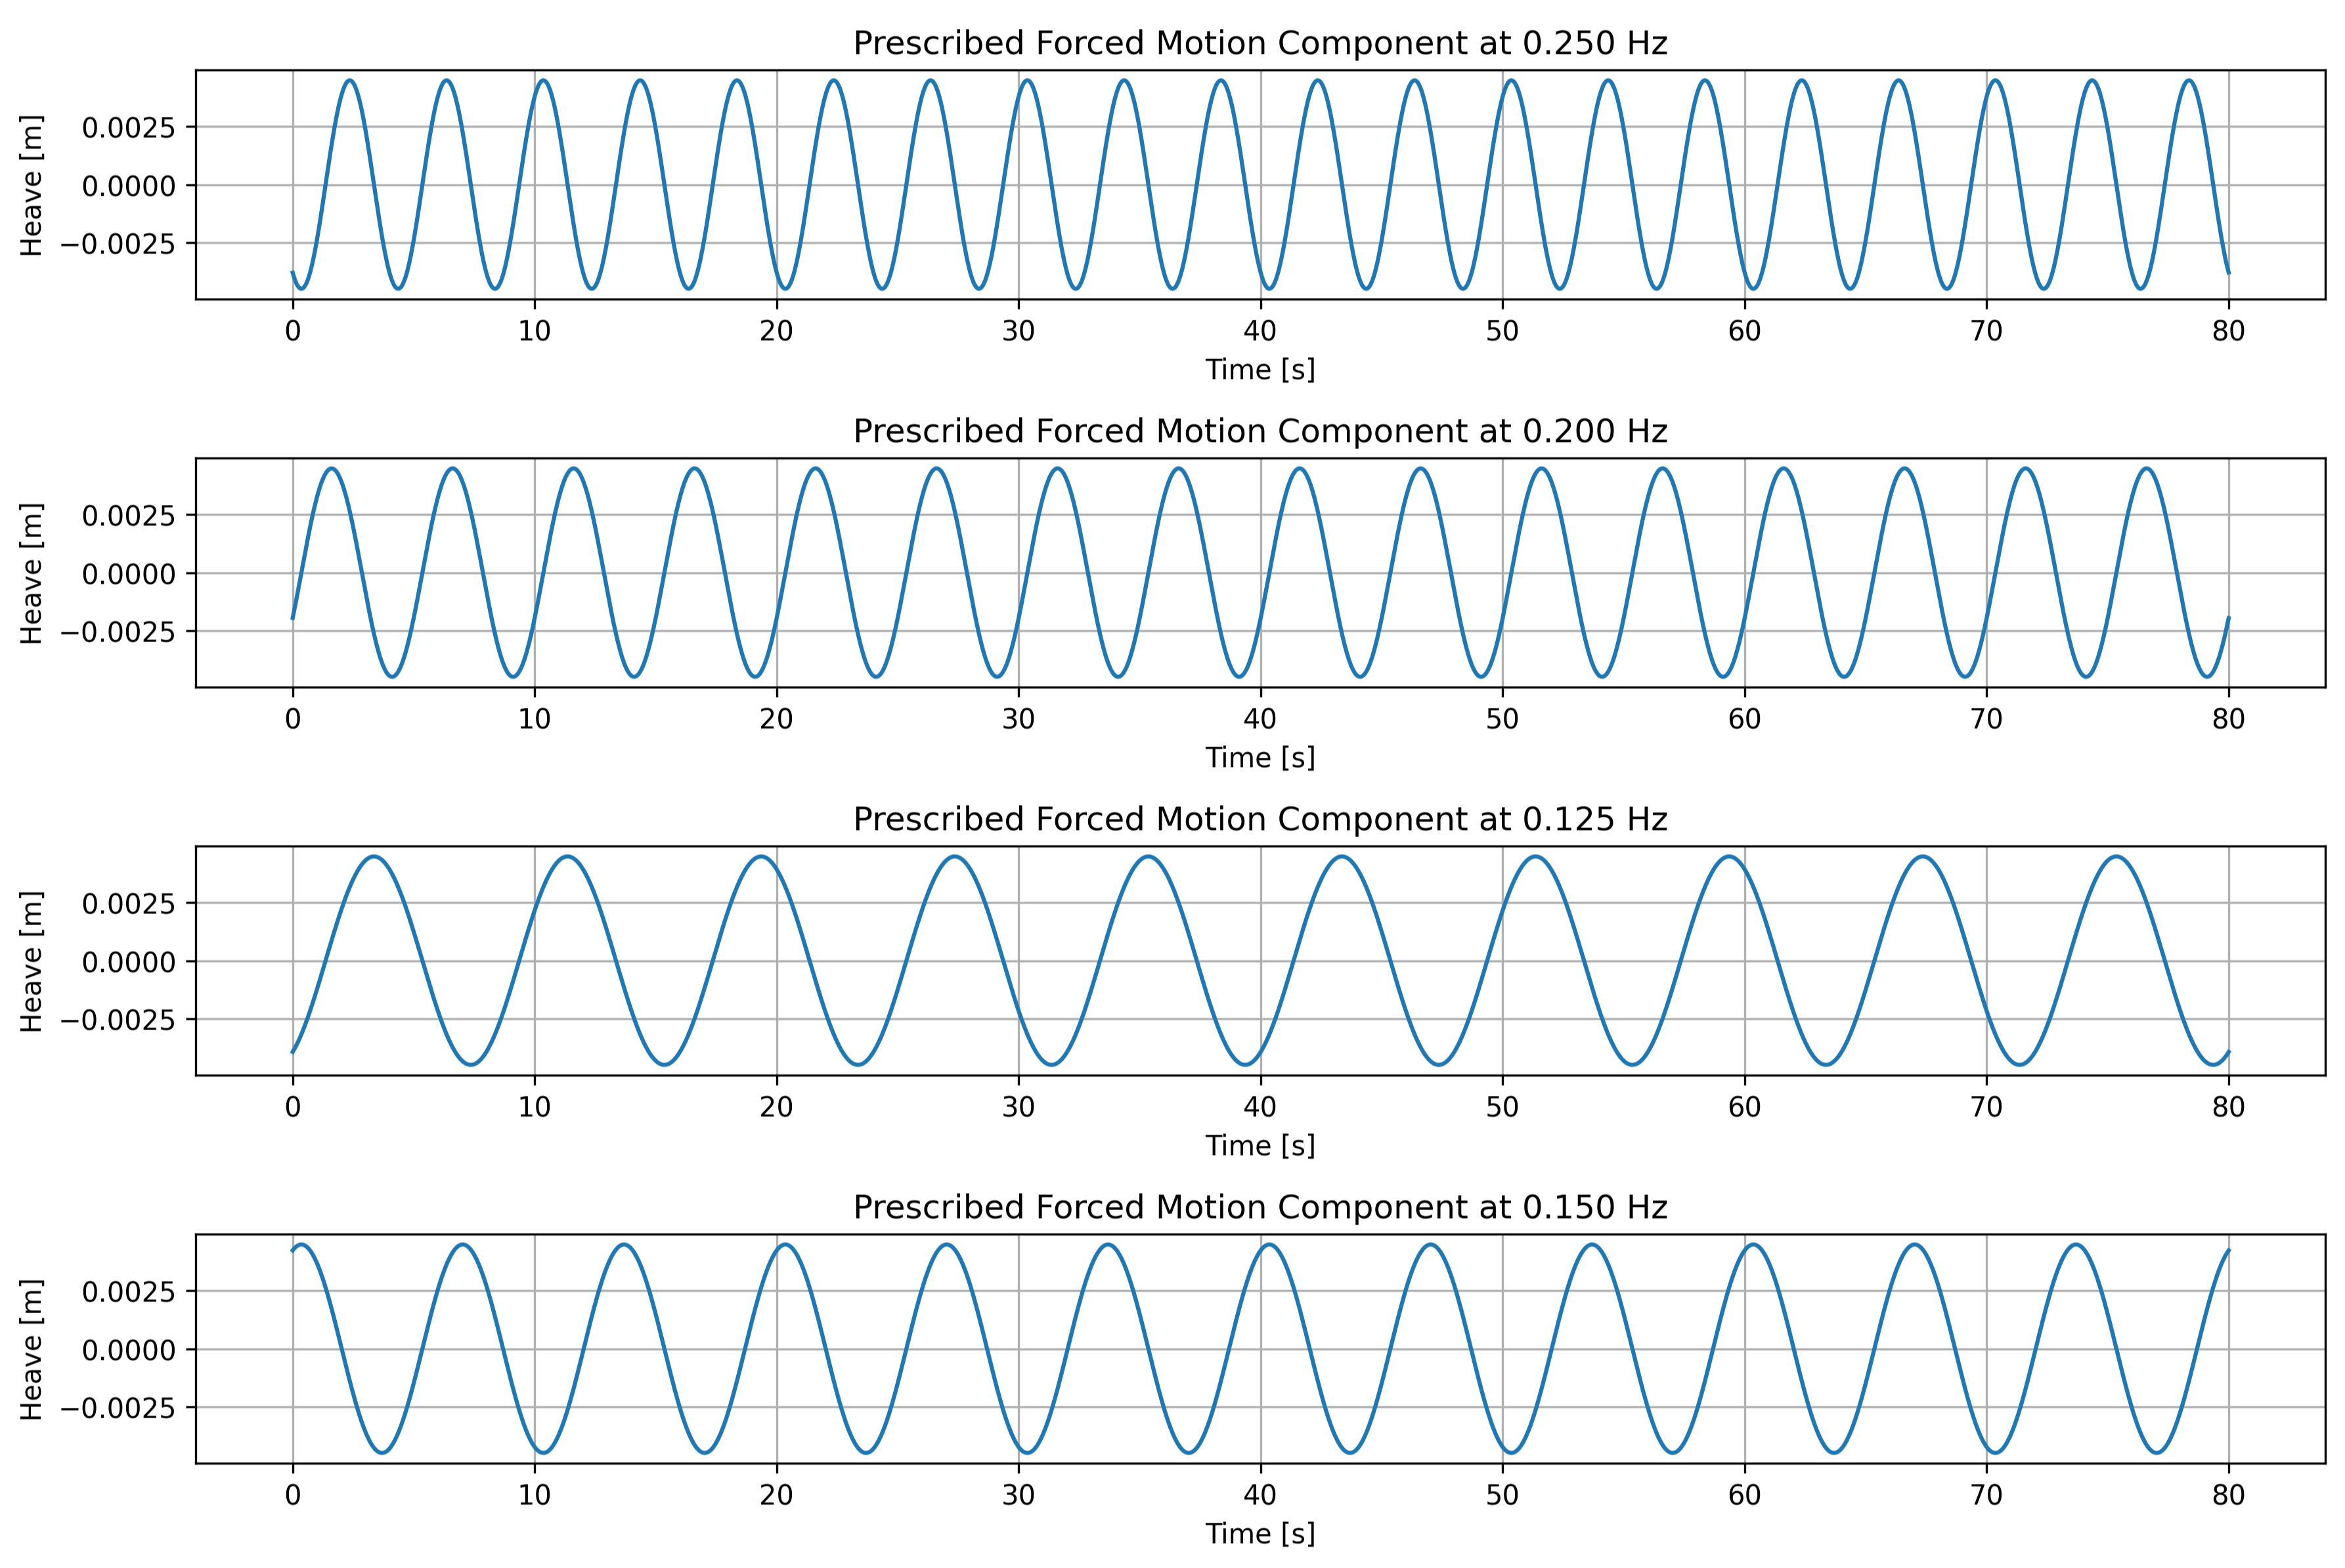
\includegraphics[width=1\textwidth]{Figures/MultiFrequency_Study_1/Procedure_Explanation/2_Individual_Component_ForcedMotion.PNG}
    \caption{Individual forced motion components for MF1 Simulation~16}
    \label{fig:MF1_IndividualComponents_ForcedMotion}
\end{figure}

These four prescribed forced motions are superposed, and the resulting superposed signal is shown in Figure~\ref{fig:MF1_Superposed_ForcedMotion}.

\begin{figure}[htbp]
    \centering
    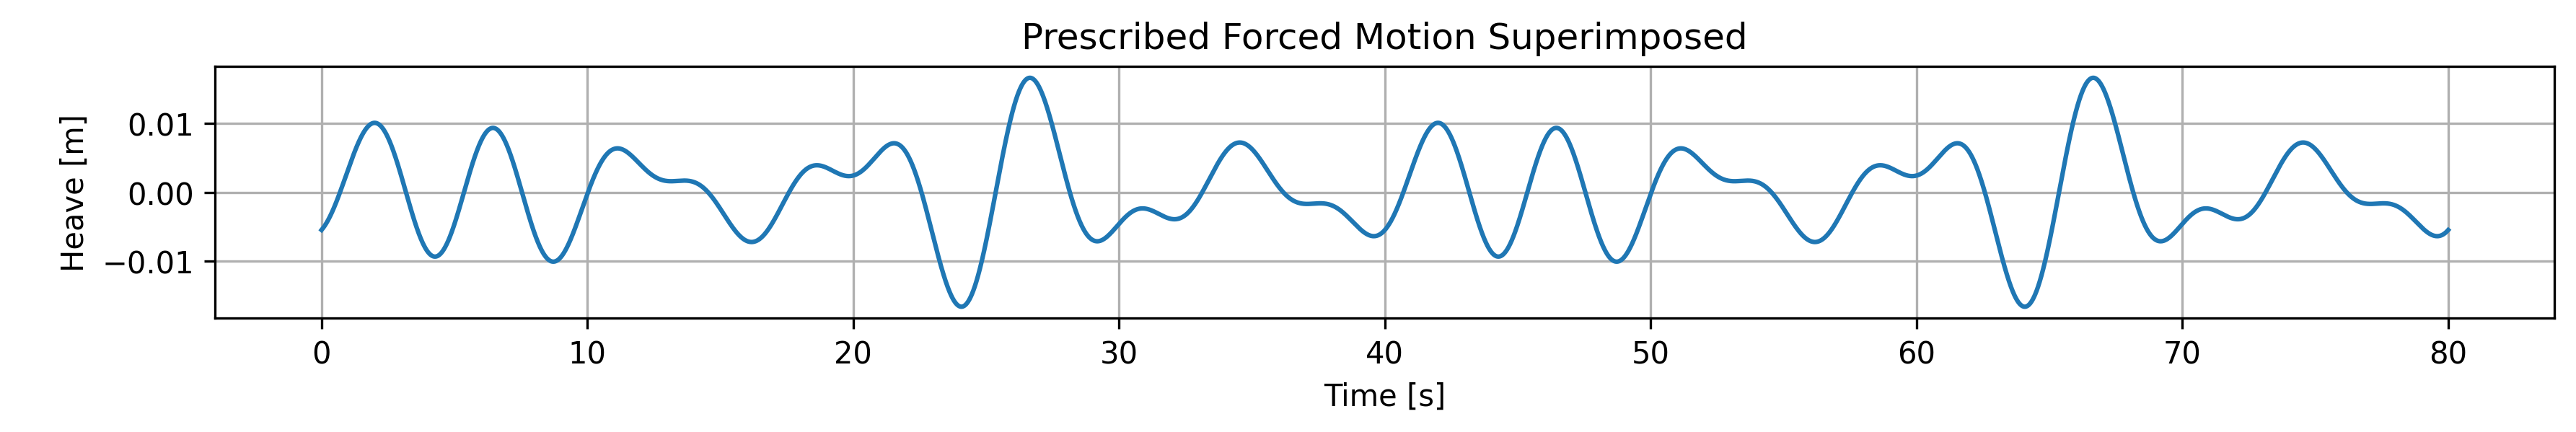
\includegraphics[width=1\textwidth]{Figures/MultiFrequency_Study_1/Procedure_Explanation/2_Superimposed_ForcedMotion.png}
    \caption{Superposed forced motion for MF1 Simulation~16}
    \label{fig:MF1_Superposed_ForcedMotion}
\end{figure}

This superposed forced motion is applied to the bridge deck in CFD, and the resulting aerodynamic lift 
and moment forces are measured. The CFD pressure is integrated over the surface to obtain the aerodynamic 
lift and moment. The computed aerodynamic lift and moment for MF1 Simulation~16 (heave) are shown in 
Figures~\ref{fig:MF1_AeroLift_TimeDomain} and~\ref{fig:MF1_AeroMoment_TimeDomain}, respectively.\\

\begin{figure}[htbp]
    \centering
    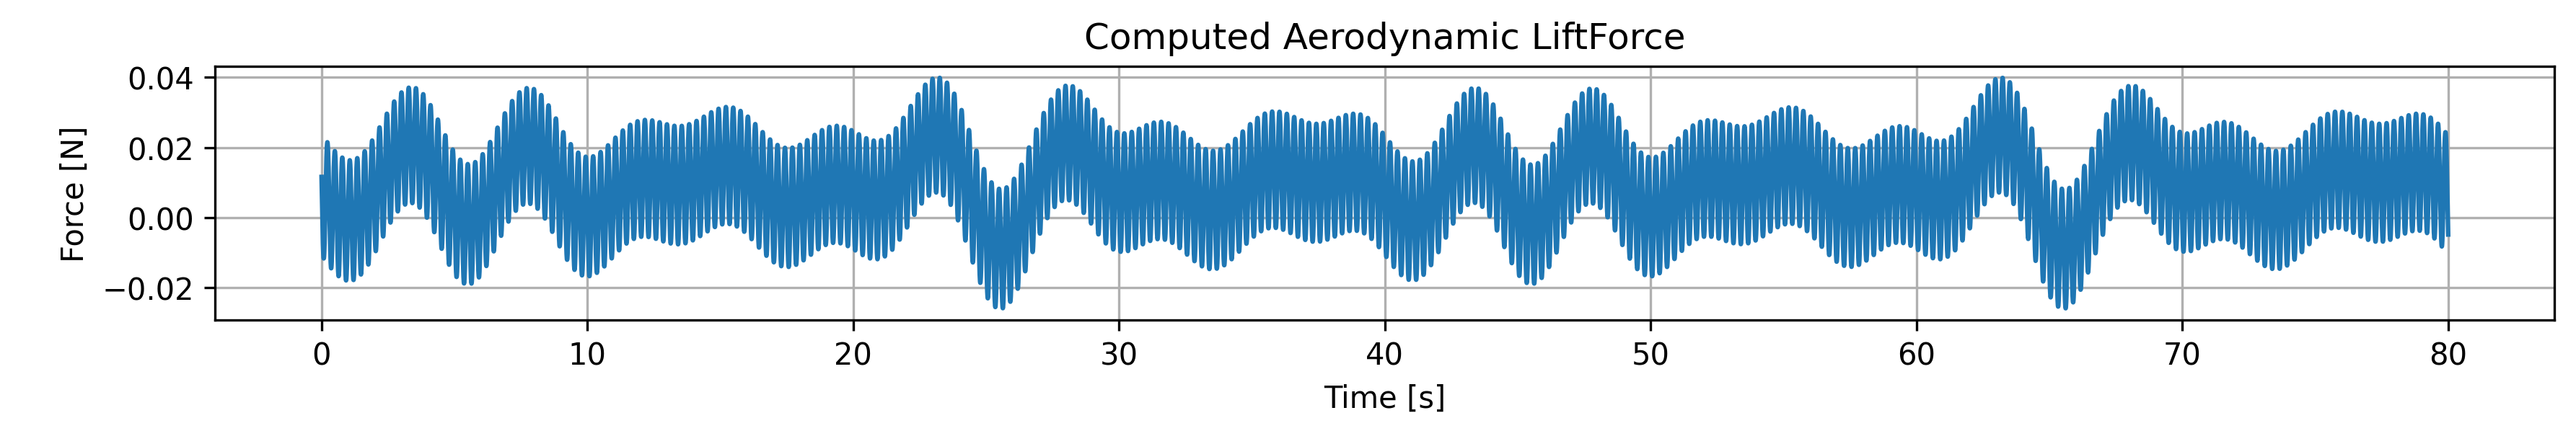
\includegraphics[width=1\textwidth]{Figures/MultiFrequency_Study_1/Procedure_Explanation/3_Computed_Aerodynamic_Lift_Force.png}
    \caption{Aerodynamic lift force in the time domain - MF1 Simulation~16}
    \label{fig:MF1_AeroLift_TimeDomain}
\end{figure}

The lift force is then transformed into the frequency domain using the FFT tool, and the result is shown 
in Figure~\ref{fig:MF1_DFT_LiftForce_SP4}.

\begin{figure}[htbp]
    \centering
    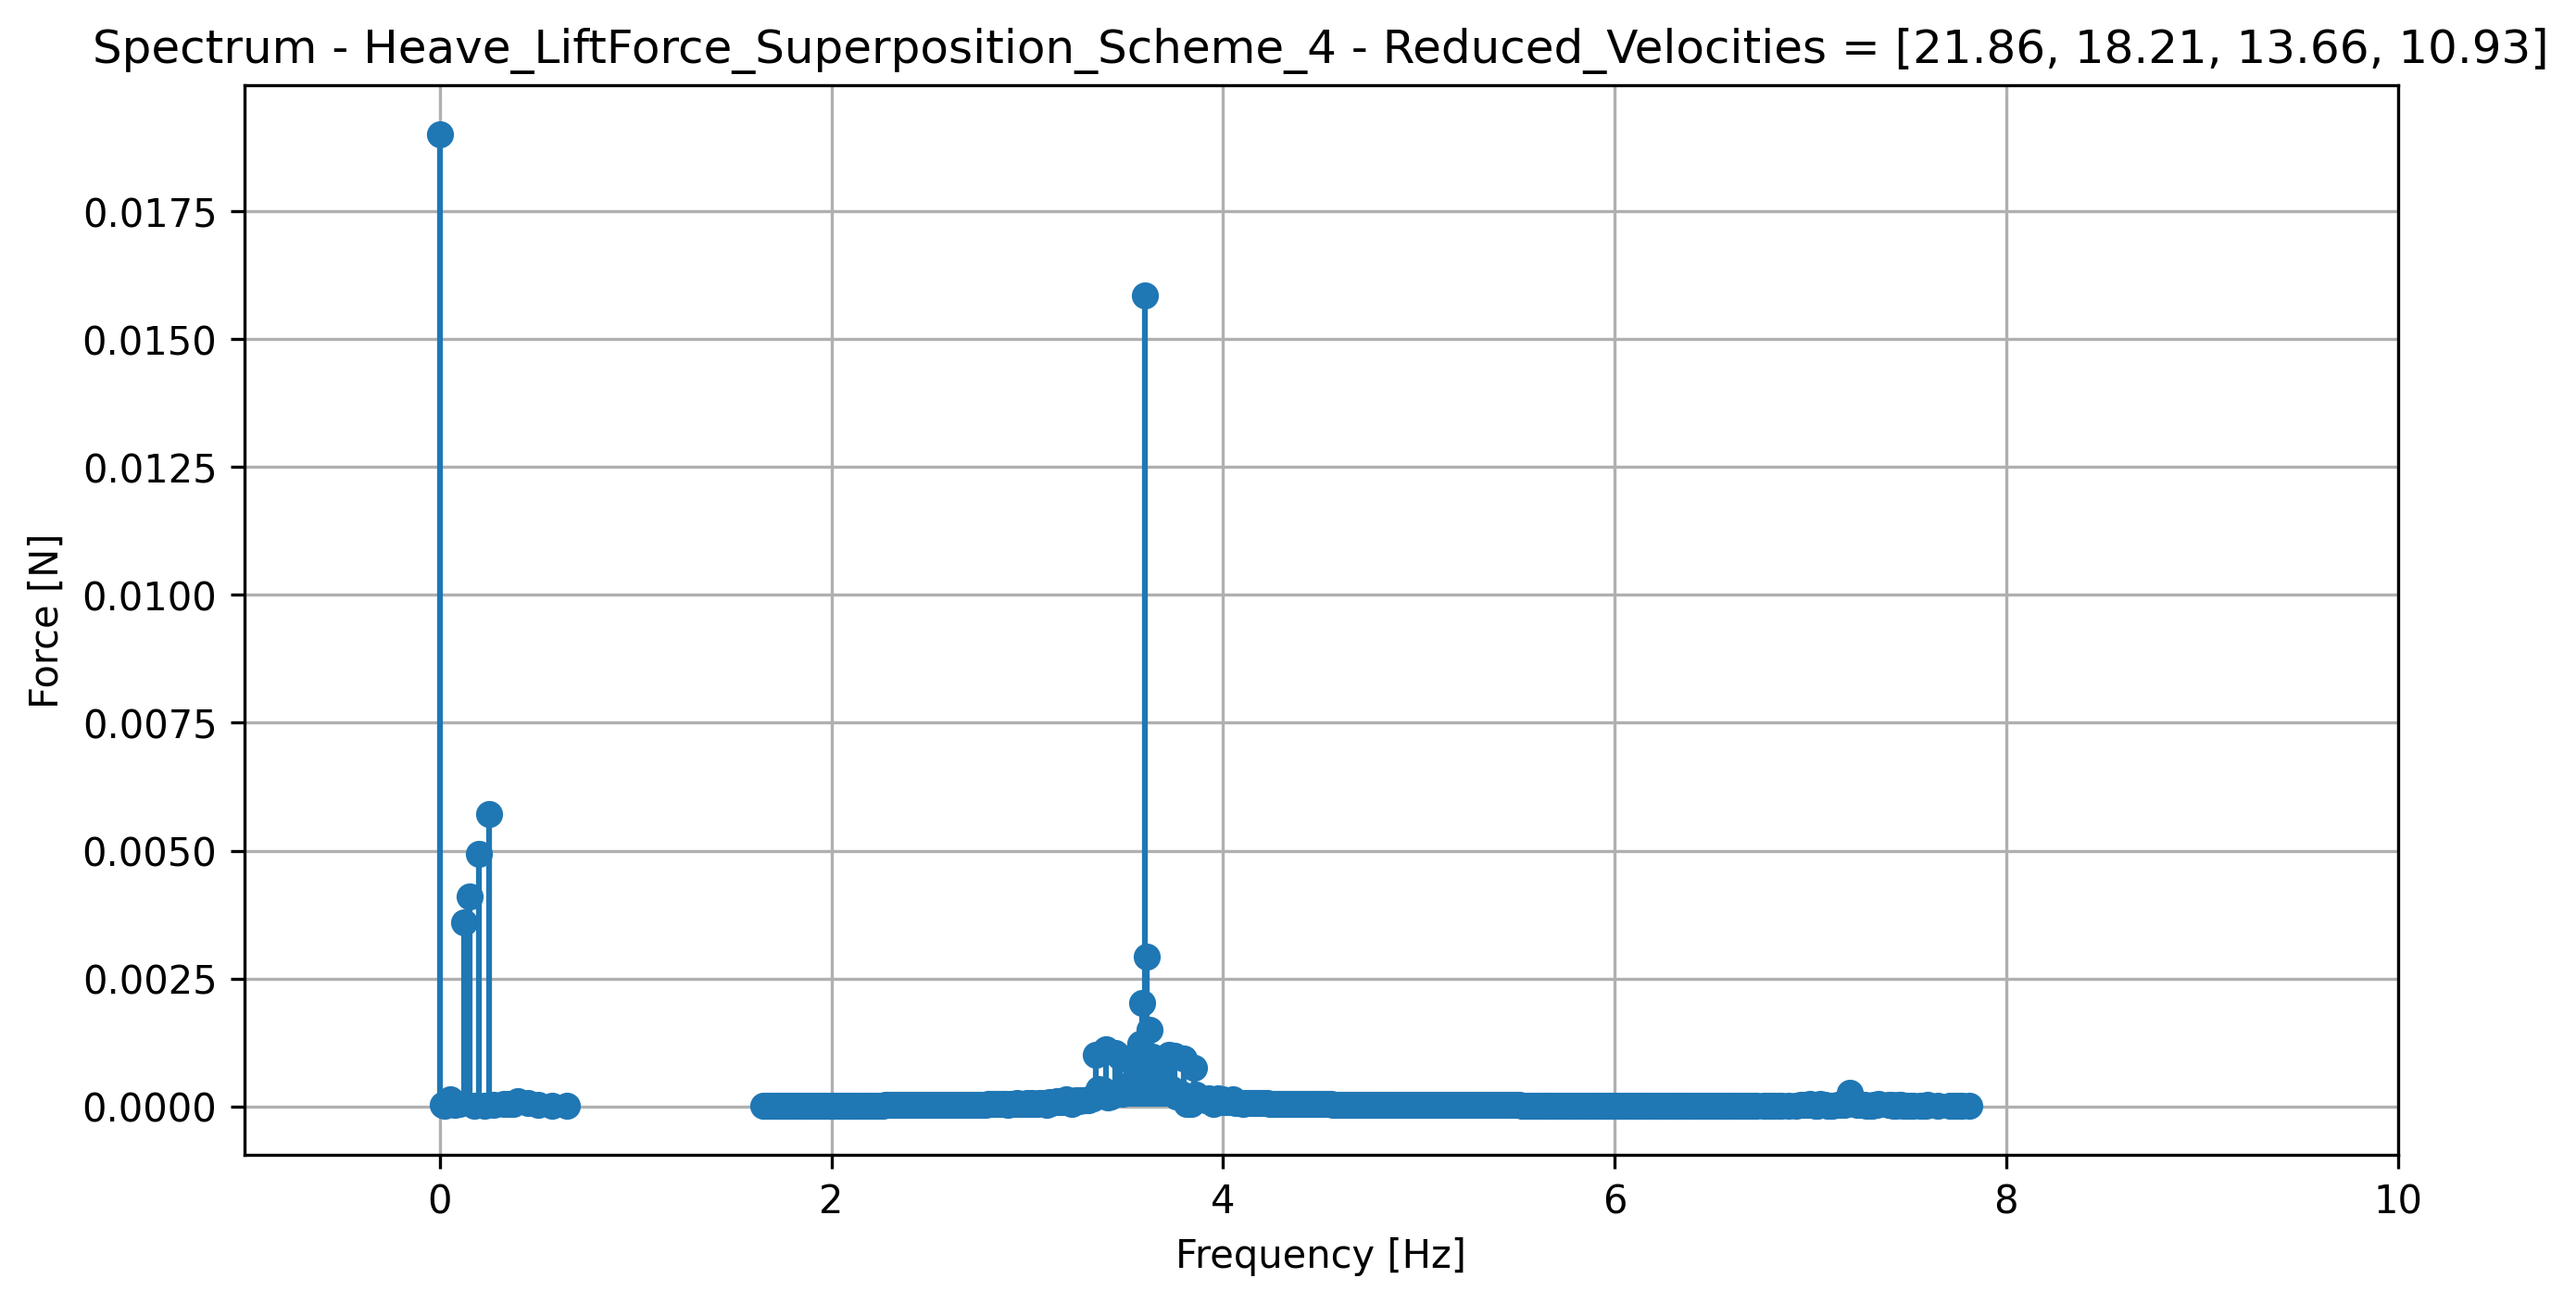
\includegraphics[width=0.6\textwidth]{Figures/MultiFrequency_Study_1/Procedure_Explanation/3_DFT_LiftForce_Superposition_Scheme_4.png}
    \caption{Aerodynamic lift force in the frequency domain - MF1 Simulation~16}
    \label{fig:MF1_DFT_LiftForce_SP4}
\end{figure}

Six peaks are visible in total. The first peak at 0~Hz corresponds to the static aerodynamic lift force 
component of the section. The following four consecutive peaks correspond to the individual aerodynamic force 
components at each prescribed frequency. The final peak at approximately 3.6~Hz corresponds to the vortex shedding frequency.\\

The individually extracted aerodynamic lift force components are shown in Figure~\ref{fig:MF1_IndividualHarmonicLift}. 
The corresponding amplitude and phase values are listed in Table~\ref{tab:MF1_AmpPhase_SP4}. 
The equivalent results for the aerodynamic moment are shown in 
Figures~\ref{fig:MF1_AeroMoment_TimeDomain}--\ref{fig:MF1_IndividualHarmonicMoment} and Table~\ref{tab:MF1_AmpPhase_SP4}.\\

\begin{figure}[htbp]
    \centering
    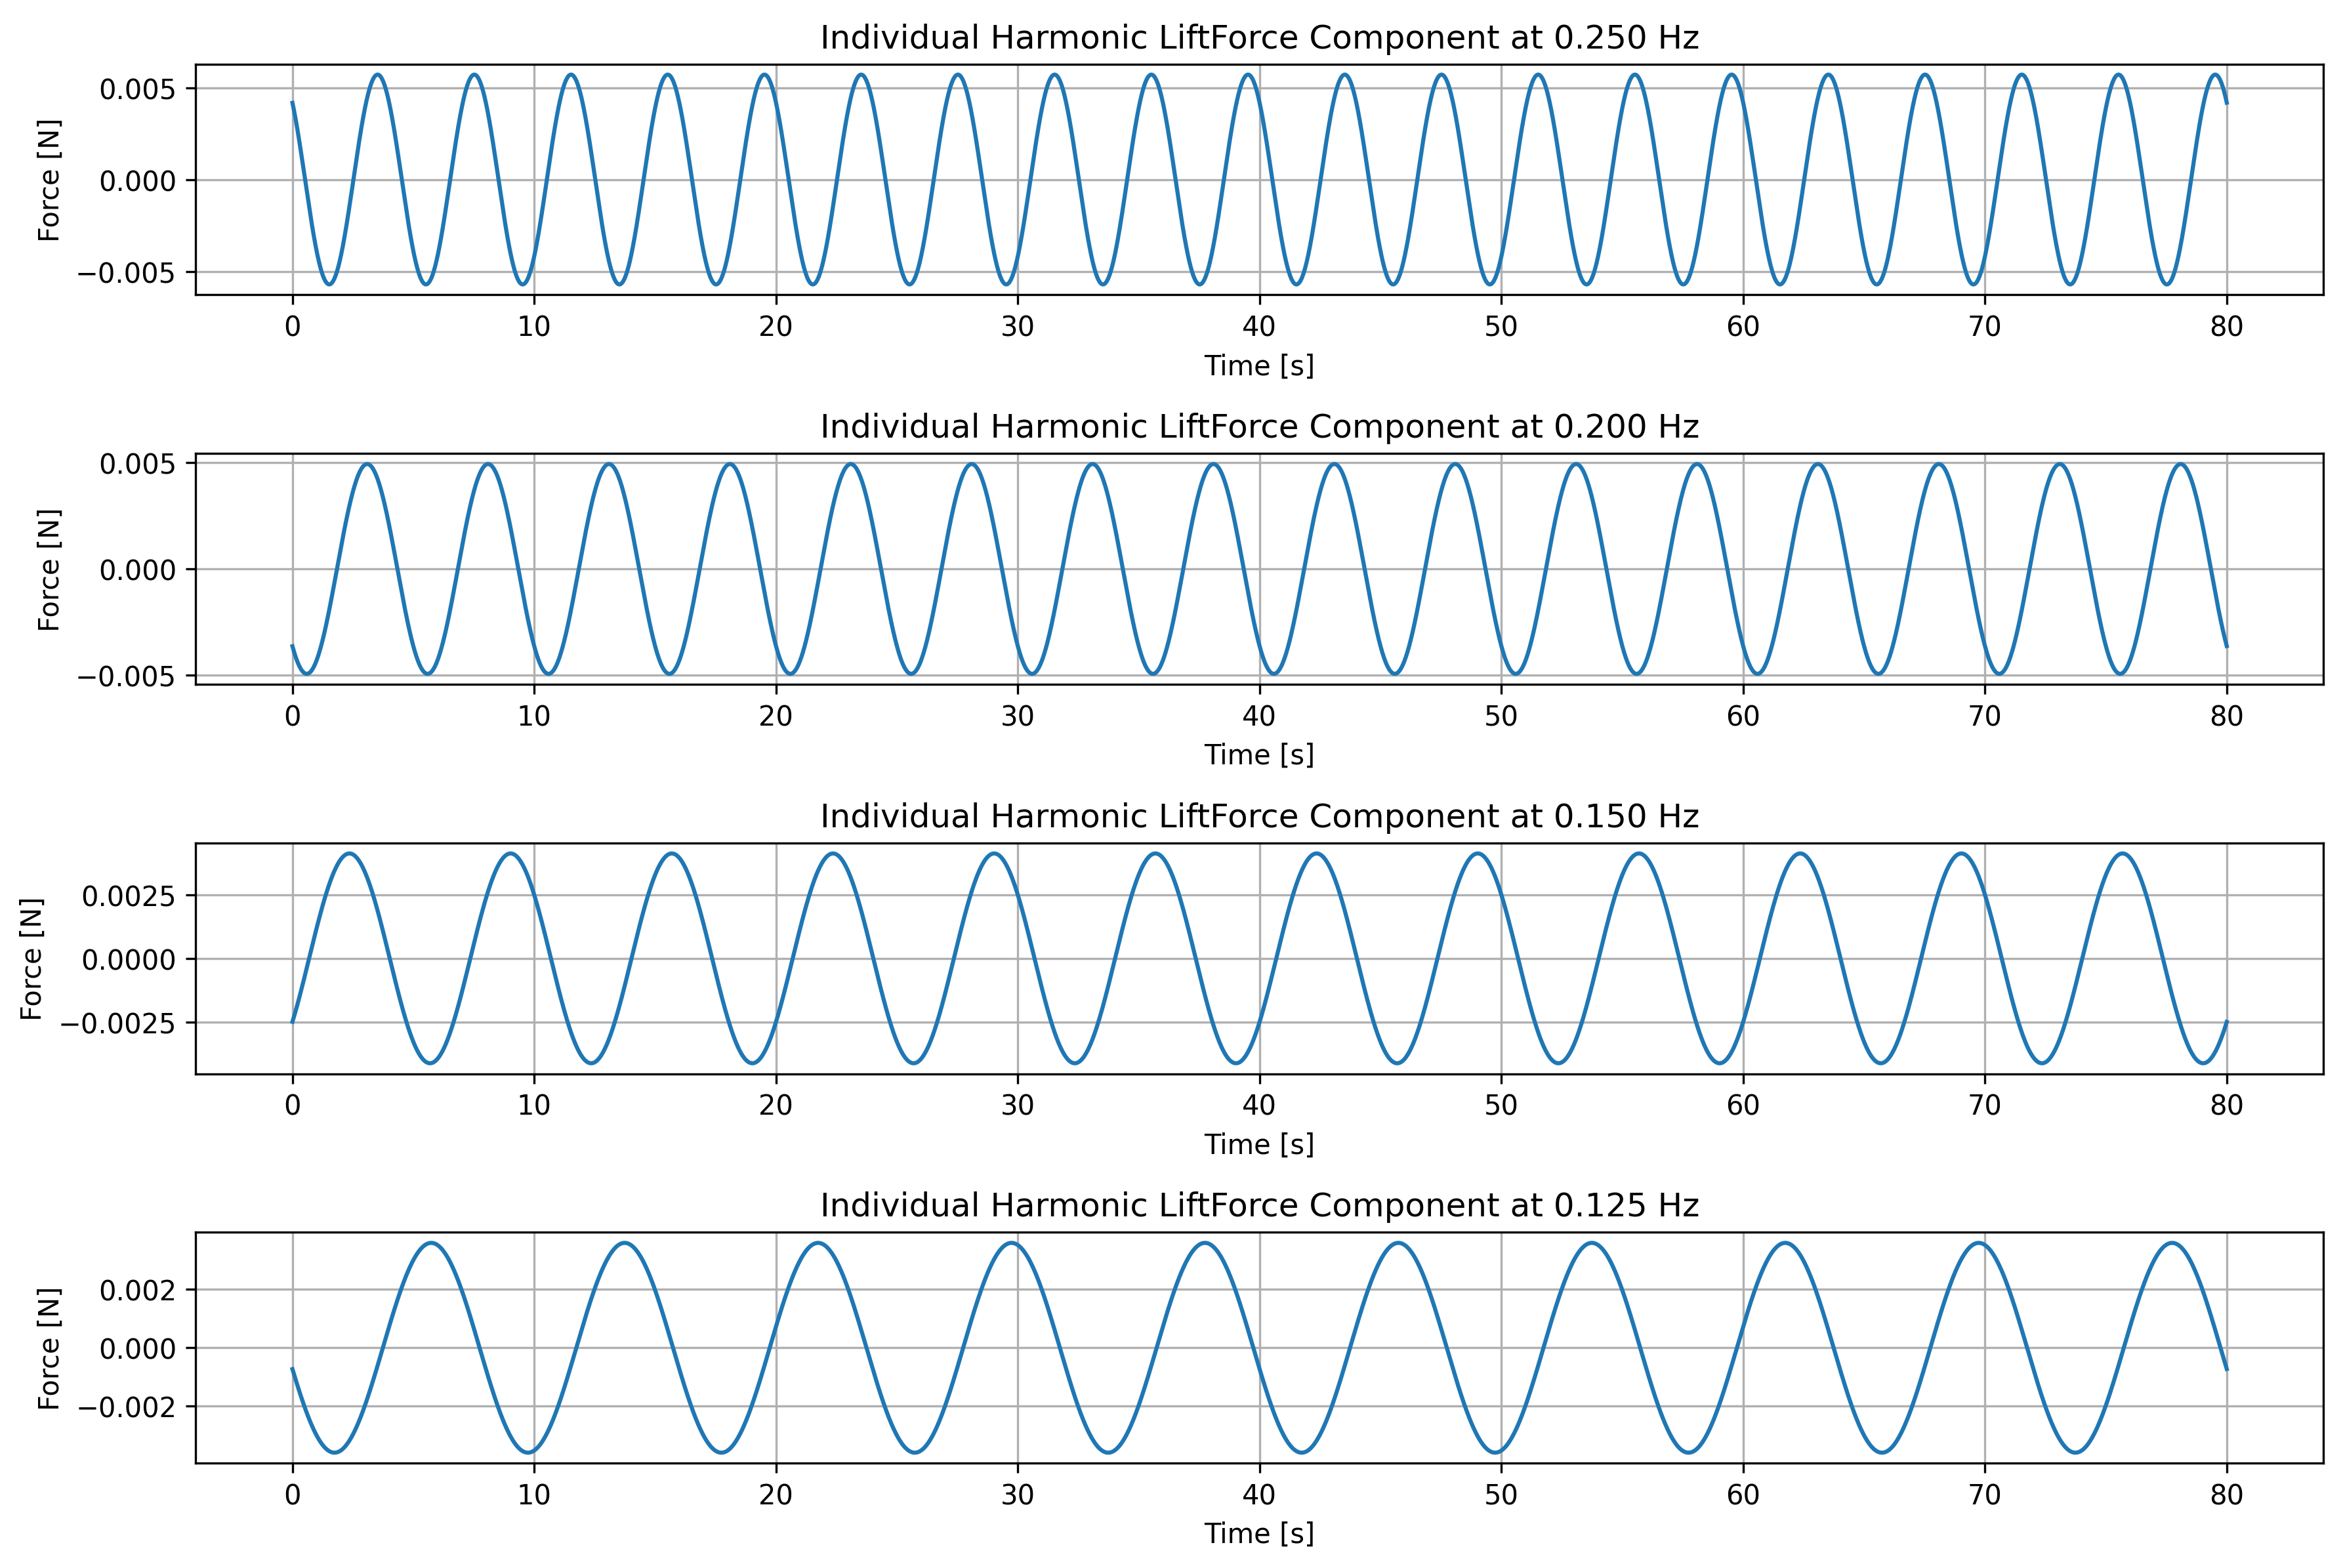
\includegraphics[width=1\textwidth]{Figures/MultiFrequency_Study_1/Procedure_Explanation/3_Individual_Harmonic_Lift_Force.png}
    \caption{Individually extracted aerodynamic lift force components - MF1 Simulation~16}
    \label{fig:MF1_IndividualHarmonicLift}
\end{figure}

\begin{figure}[htbp]
    \centering
    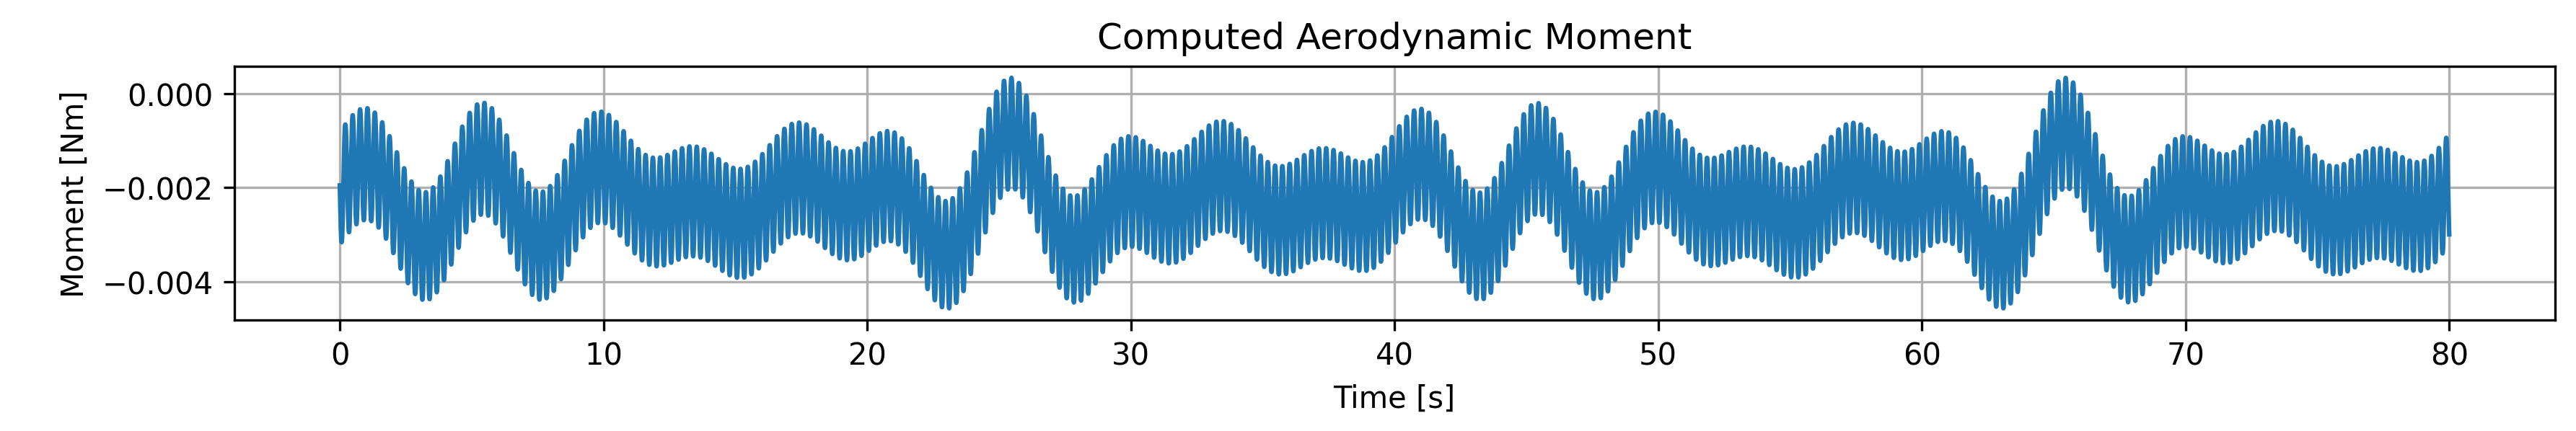
\includegraphics[width=1\textwidth]{Figures/MultiFrequency_Study_1/Procedure_Explanation/4_Computed_Aerodynamic_Moment.png}
    \caption{Aerodynamic moment in the time domain - MF1 Simulation~16}
    \label{fig:MF1_AeroMoment_TimeDomain}
\end{figure}

\begin{figure}[htbp]
    \centering
    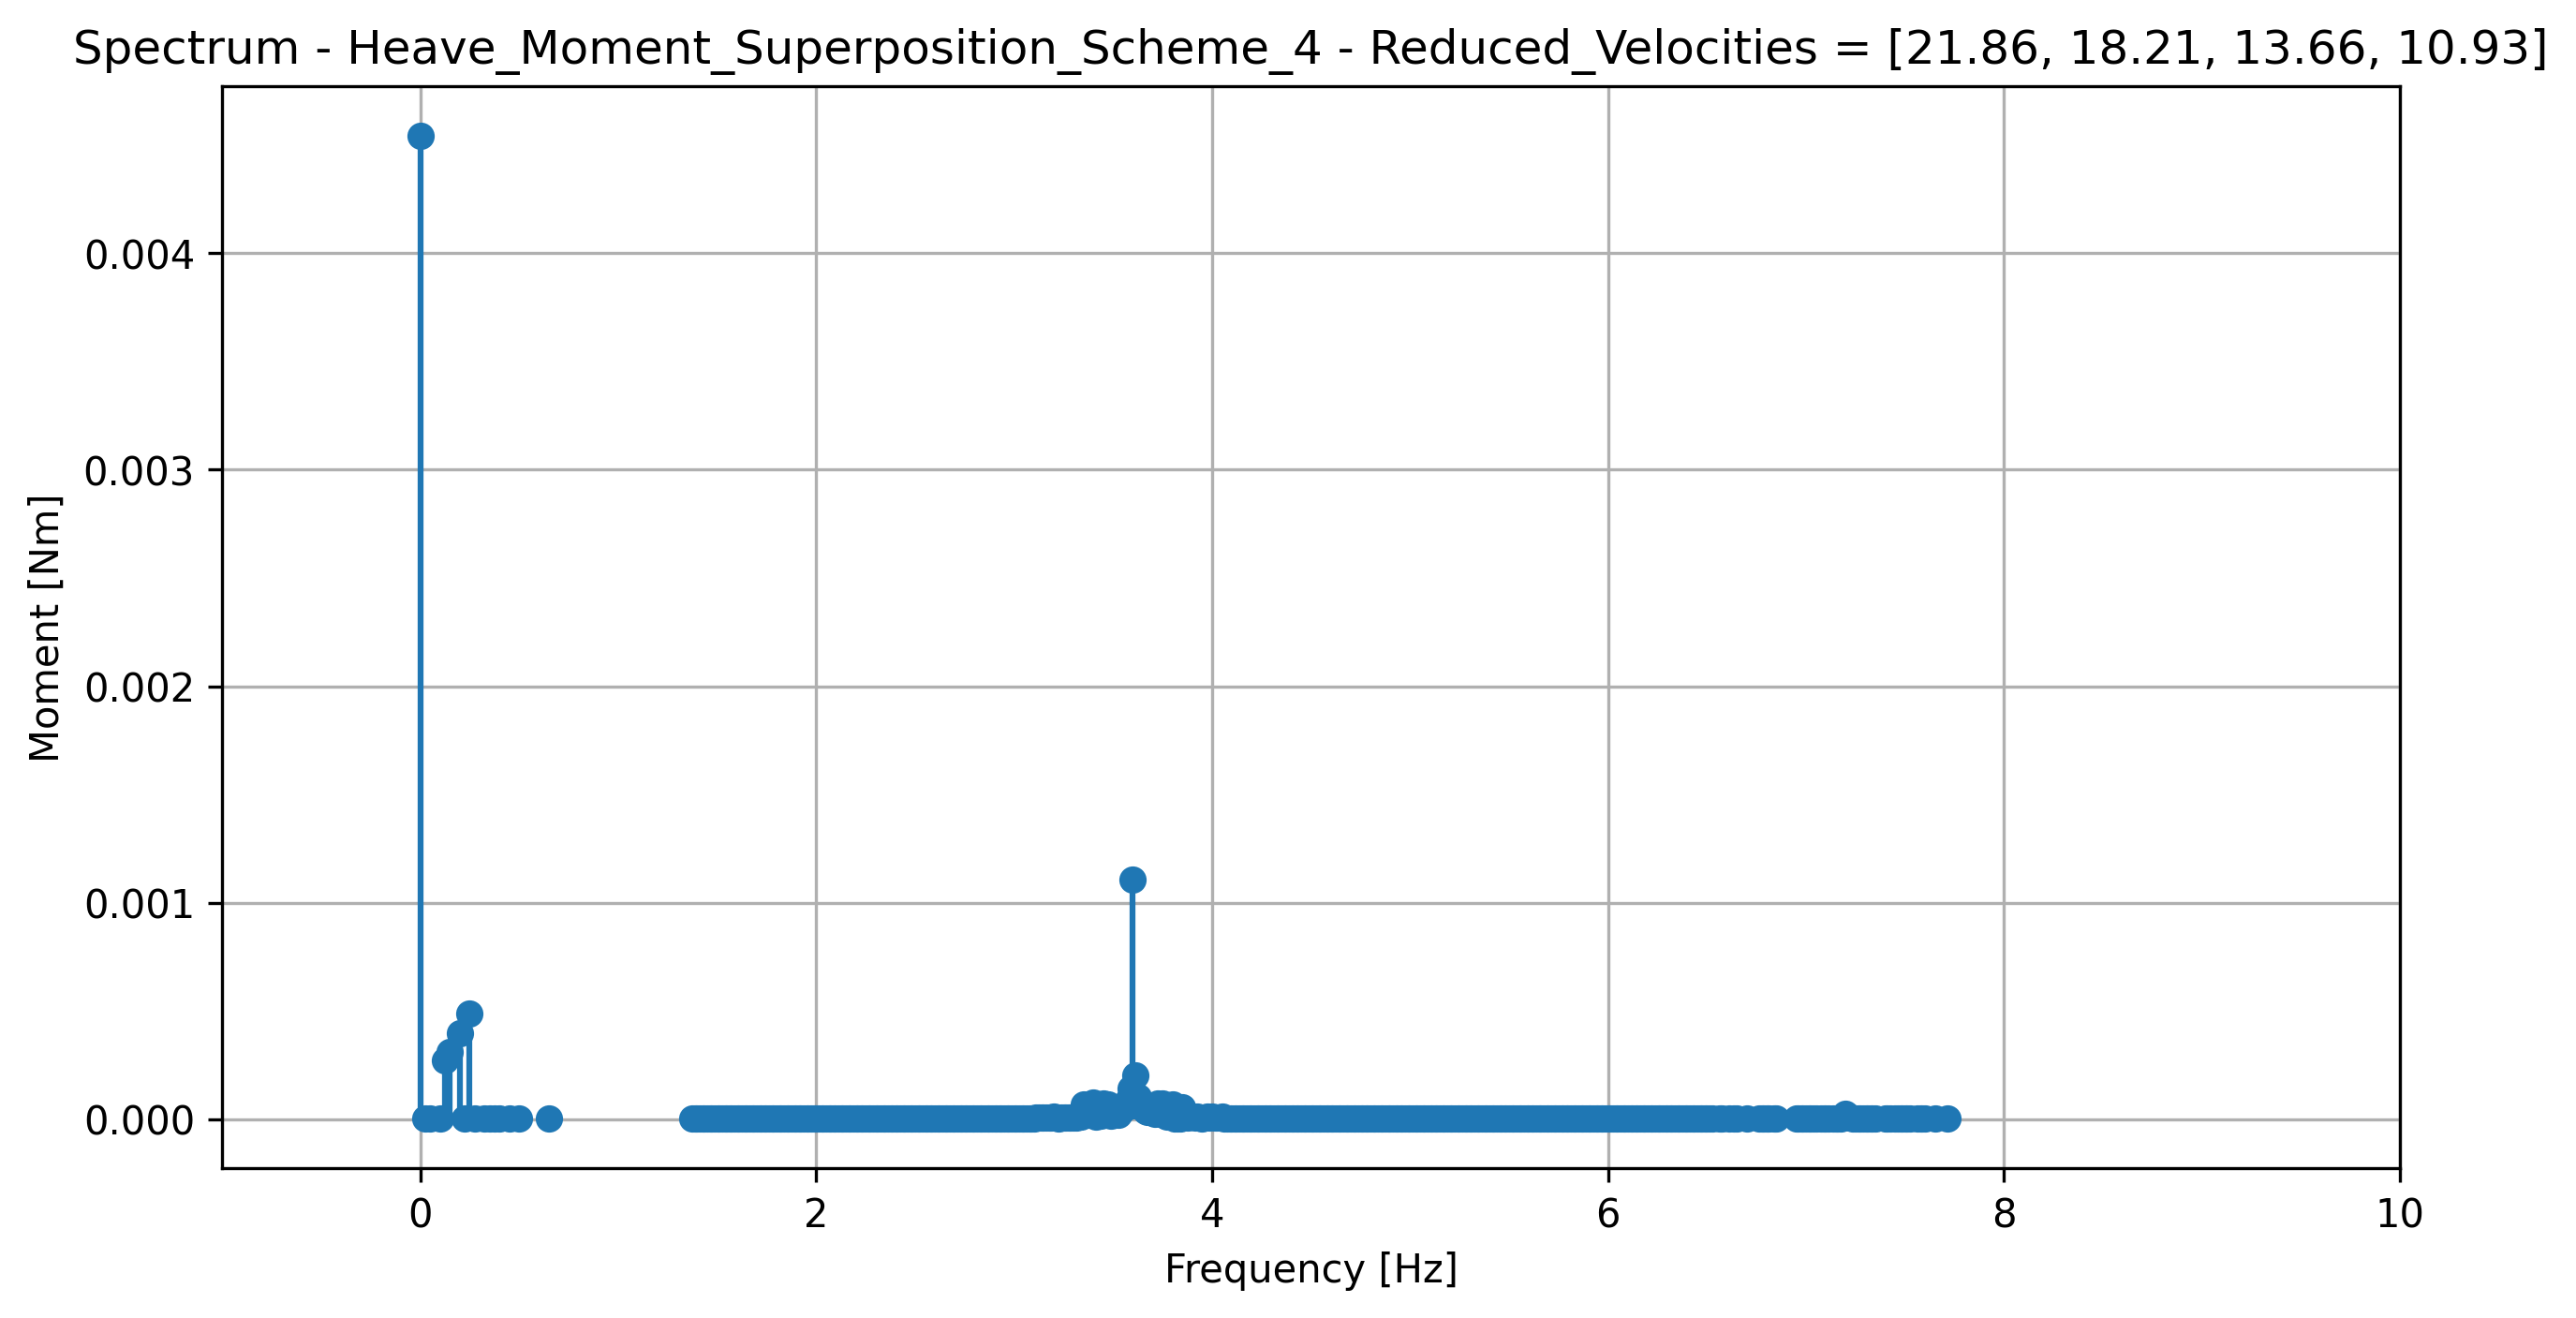
\includegraphics[width=0.6\textwidth]{Figures/MultiFrequency_Study_1/Procedure_Explanation/4_DFT_Moment_Superposition_Scheme_4.png}
    \caption{Aerodynamic moment in the frequency domain - MF1 Simulation~16}
    \label{fig:MF1_DFT_Moment_SP4}
\end{figure}

\begin{figure}[htbp]
    \centering
    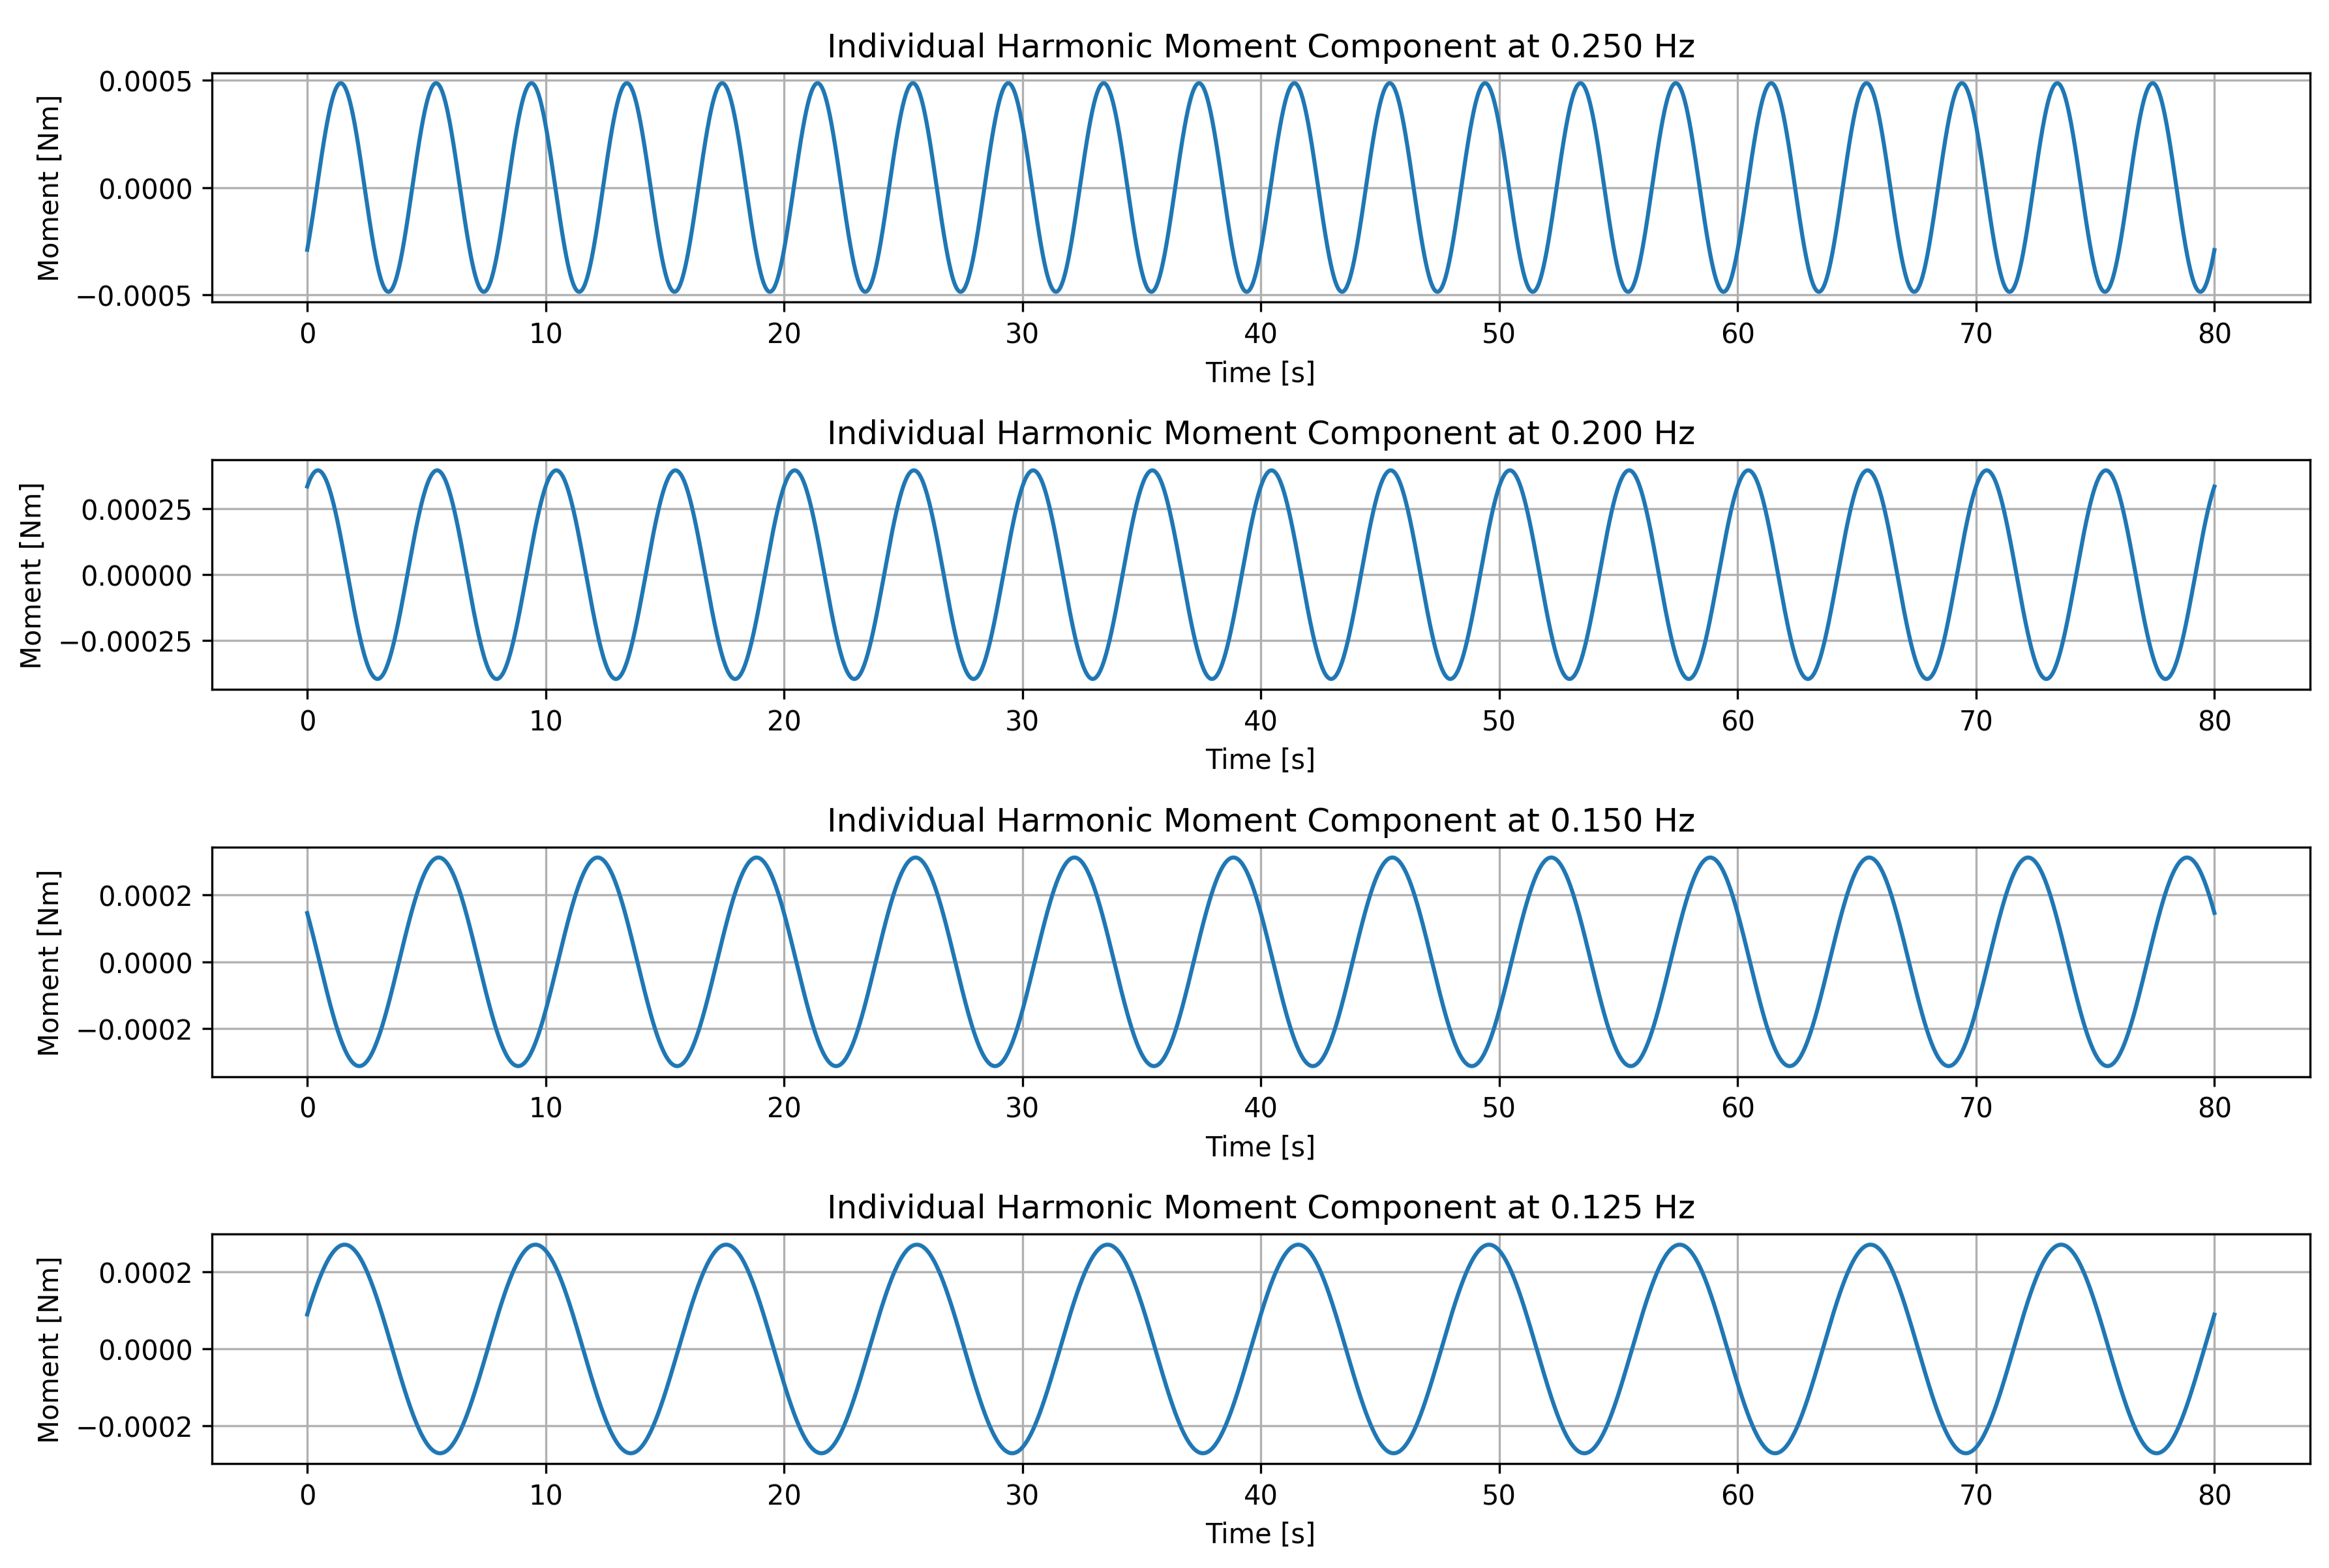
\includegraphics[width=1\textwidth]{Figures/MultiFrequency_Study_1/Procedure_Explanation/4_Individual_Harmonic_Moment.png}
    \caption{Individually extracted aerodynamic moment components - MF1 Simulation~16}
    \label{fig:MF1_IndividualHarmonicMoment}
\end{figure}

\begin{table}[htbp]
\centering
\caption{Amplitude and Phase Data for MF1 Simulation~16 (Heave, Superposition~4)}
\label{tab:MF1_AmpPhase_SP4}
\begin{tabular}{|l|c|c|c|c|c|}
\hline
\rule{0pt}{12pt}\textbf{Frequency} 
    & \textbf{LiftForce($F_y$) N} 
    & \textbf{$F_y$ Phase rad} 
    & \textbf{Moment($M_x$) Nm}
    & \textbf{$M_x$ Phase rad} \\[4pt]
\hline
0.125 & 0.003595 & 1.8699 & 0.000271 & -1.4036 \\
0.15  & 0.004113 & 1.8826 & 0.000311 & -1.4219 \\
0.2   & 0.004939 & 1.8631 & 0.000396 & -1.4578 \\
0.25  & 0.005710 & 1.8276 & 0.000486 & -1.4930 \\
\hline
\end{tabular}
\end{table}

\subsection{Flutter Derivatives Results and Comparison}

\begin{figure}[htbp]
    \centering
    
\includegraphics[width=1\textwidth]{Figures/MultiFrequency_Study_1/Combined_Flutter_Derivative.png}
    \caption{flutter derivatives - Campaign~1}
    \label{fig:Combined_Flutter_Derivatives_1}
\end{figure}

The 34 CFD simulations is conducted with LRZ High Performance computer and the results discussed in the current and following sections. 
From the flutter derivatives plot (Figure~\ref{fig:Combined_Flutter_Derivatives_1}) 
it can be observed that $H_1$, $A_1$, $H_3$, $A_3$, $H_4$, and $A_4$ 
agree well across all superposition schemes. For superposition scheme~4, a slight error is 
introduced, which is located in the lower reduced velocity range (i.e.\ below $U_r = 6.83$). 
Due to interpolation, this error propagates to higher reduced velocities, which explains the discrepancies 
occur there.\\

It is also noted that $H_3$ and $A_3$ exhibit slightly varying values at the higher reduced velocities. 
This can be inferred from the nonlinearity study, which indicates that $H_3$ and $A_3$ display mild 
nonlinearity at higher reduced velocities. 
It is further noted that $H_4$ and $A_4$ show slightly varying values, although the magnitude of 
the error is not clearly visible in this figure.\\

For the flutter derivatives $H_2$ and $A_2$, the errors at lower reduced velocities are very small, 
even for superposition scheme~4. However, at higher reduced velocities the error becomes significantly 
larger. Based on the nonlinearity study, this is expected, as it reflects the inherent nonlinearity (due to phase of moment) of 
the flutter derivative coefficients $H_2$ and $A_2$, and is not a consequence of the multi-frequency method itself.\\

Overall, this plot indicates that, provided the multi-frequency method adheres to the framework for 
the Fourier transformation, the errors remain small. \\


\subsection{Error Analysis of Aerodynamic Forces}

In this section, the errors are quantified. Since the source of error lies in the aerodynamic forces, 
moments, and phases (structural properties are assumed to be known), the error analysis is performed 
on the forces and phases.\\

Figure~\ref{fig: Amplitude_Errors} shows the amplitude error as a function of reduced velocity for each superposition scheme. 
For heave motion (solid lines), the errors at higher reduced velocities are very small (see Tables in appendix~\ref{app:amp_phase_errors} for values). 
Below the reduced velocity of 6.83, the error rises to up to 40\% for superposition scheme~4. The reason for 
this behaviour is investigated further in Section~\ref{sec:MF1_FreqDomain}. For pitch motion, 
slight errors are present at higher reduced velocities, which is consistent with the nonlinearity 
study and in agreement with the flutter derivative plot discussed in previous section.\\

An important inference here is that, although the total prescribed motion amplitude is the same across all four 
multi-frequency schemes, the results reflects the inherent nonlinearity of 
the cross-section. This shows the key distinction: not only must the peak amplitude be kept 
below the nonlinearity threshold, but the instantaneous amplitude at every point in time must 
also remain within this limit. This condition is satisfied only in the single-frequency case. 
Consequently, the multi-frequency method can never yield results fully equivalent to single-frequency 
analysis when the cross-section exhibits inherent nonlinearity (due to phase change), even at low amplitude ranges.\\

An important counterpoint is that, flutter derivative identifications aim 
to simulate real-world conditions, where the induced motion is not a pure single-frequency. 
From this perspective, it can be argued that the multi-frequency method provides a more 
representative result than single-frequency oscillation (because of inclusion of phase change). Therefore, 
whether the deviations in $A_2$ and $H_2$ are acceptable depends on the perspective adopted 
and the intended use of the results.\\

\begin{figure}[htbp]
    \centering
    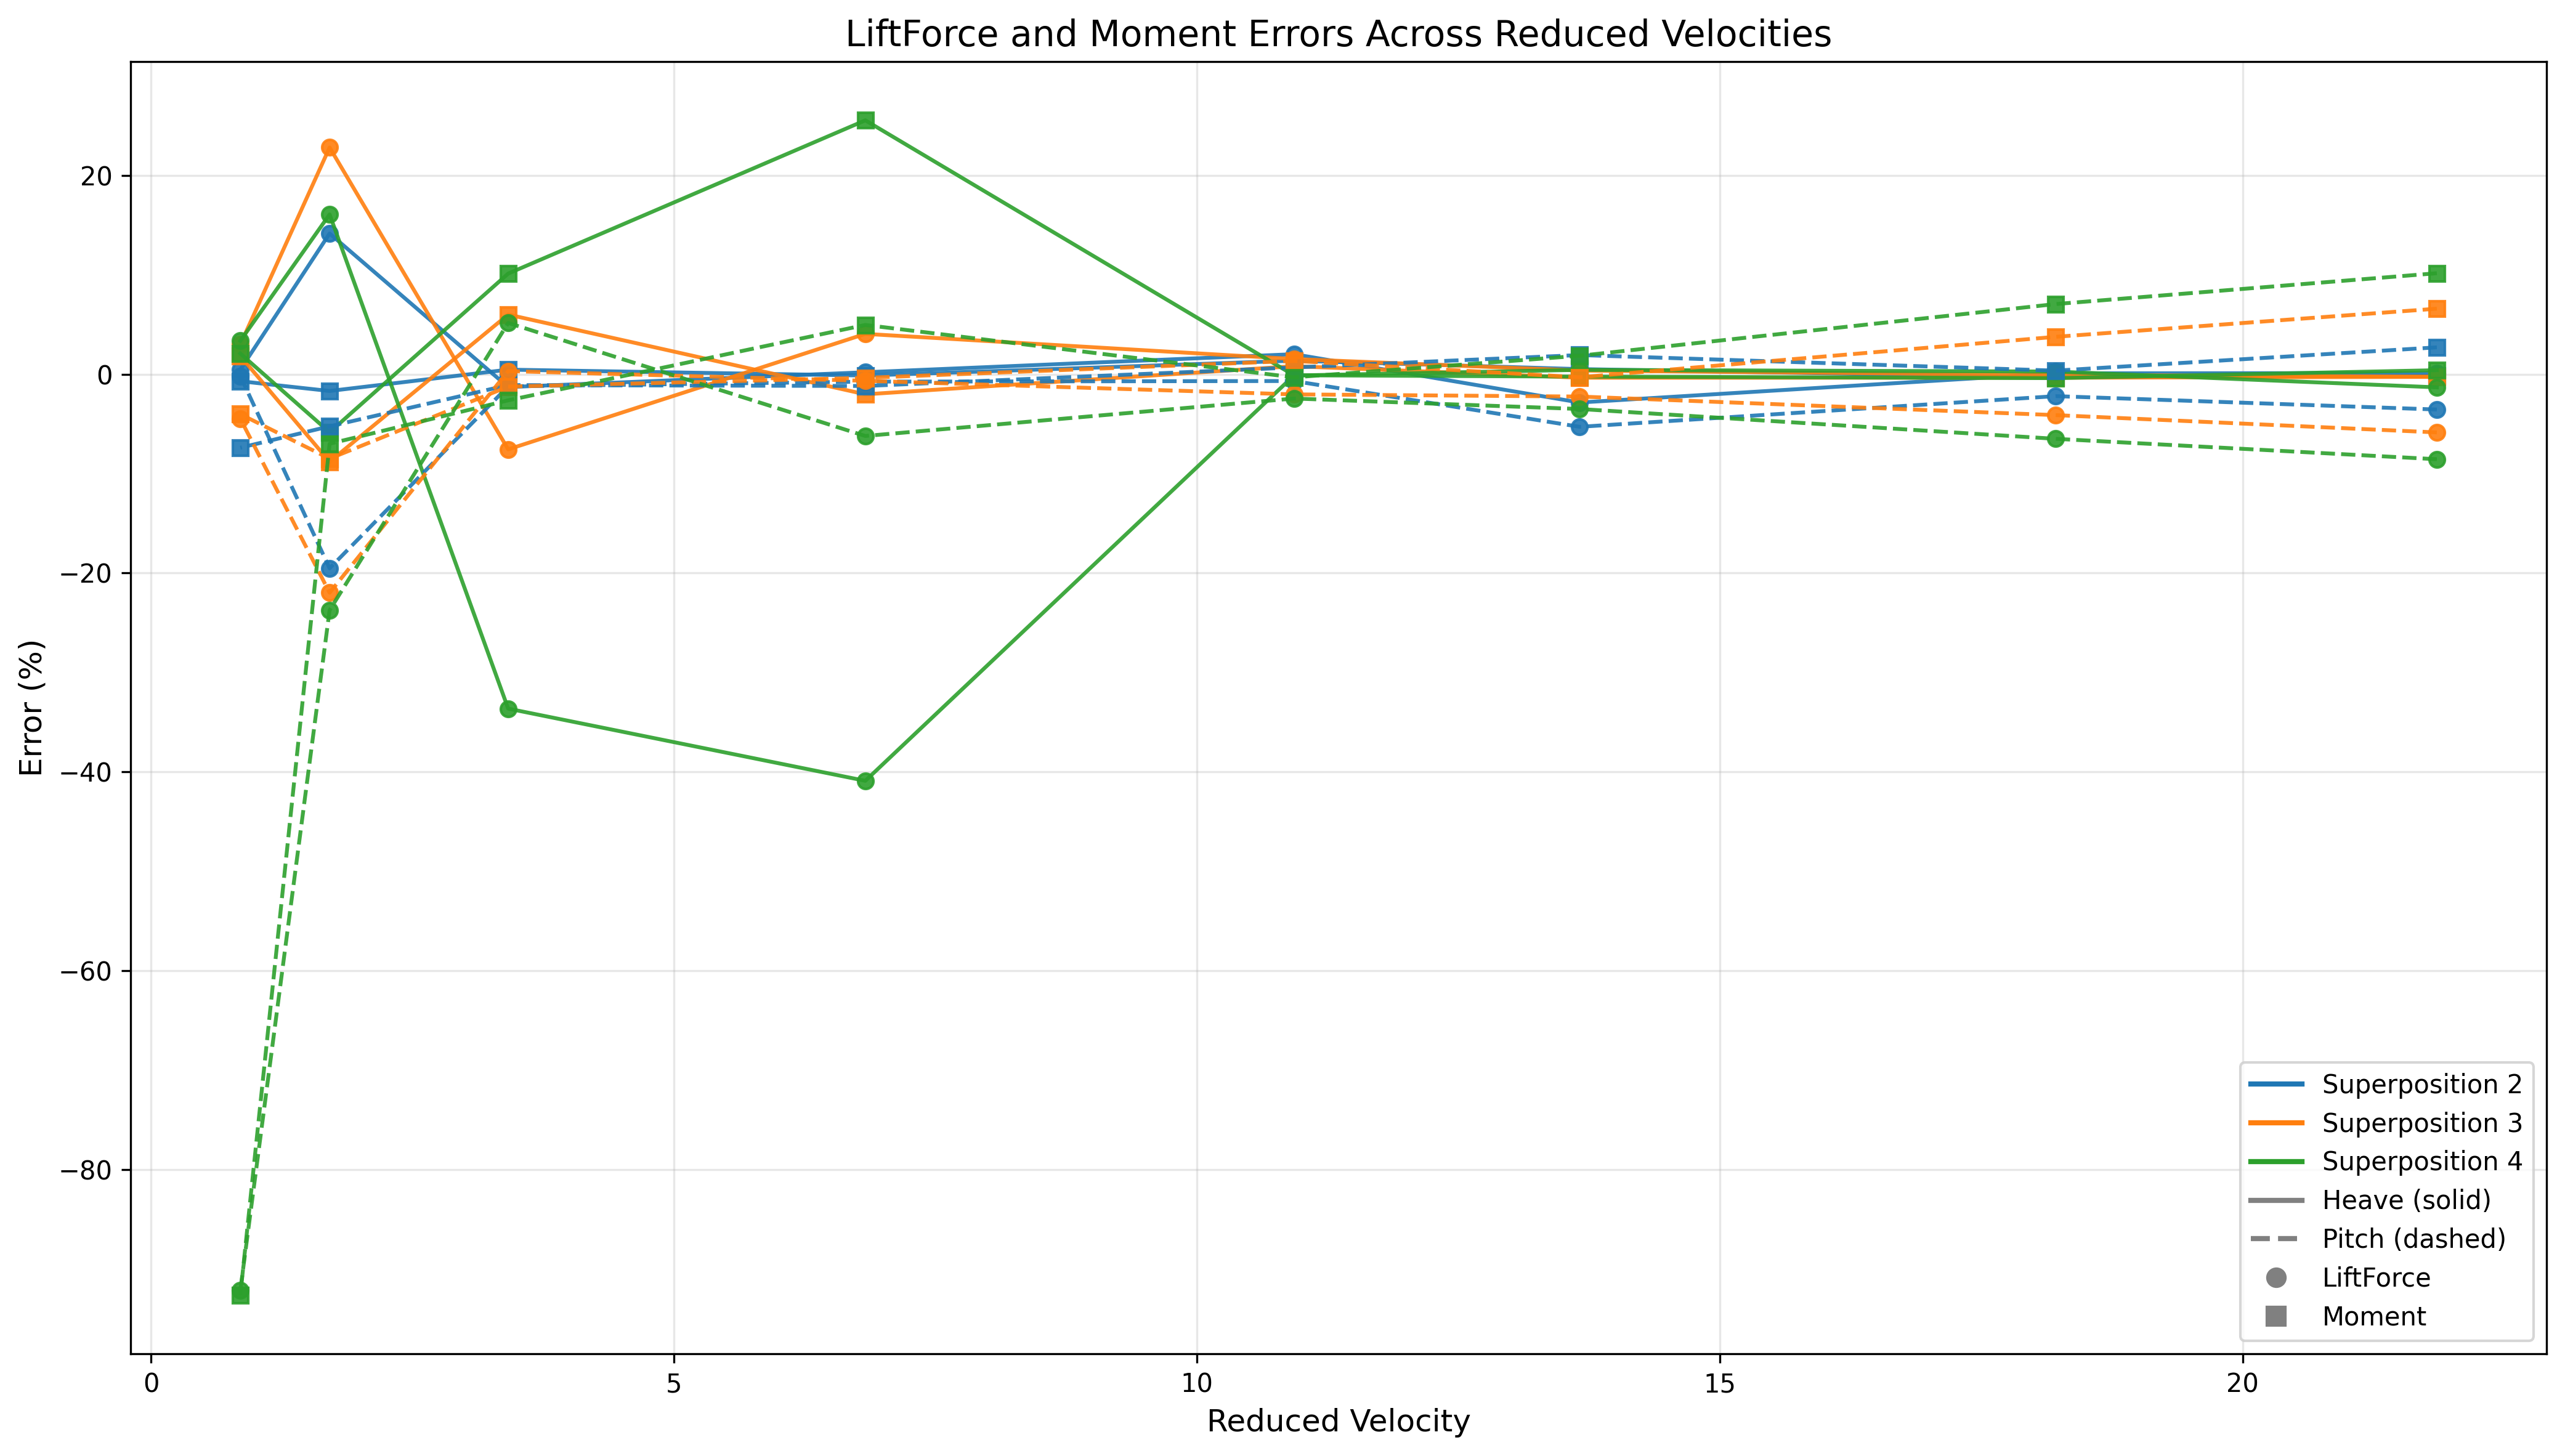
\includegraphics[width=1\textwidth]{Figures/MultiFrequency_Study_1/Combined_Amplitude_Errors.png}
    \caption{Amplitude errors as a function of reduced velocity - Campaign~1}
    \label{fig: Amplitude_Errors}
\end{figure}

From the Figure~\ref{fig: Phase_Errors}, the phase erros exist for pitch motion accross all reduced velocities. 
For heave motion, it is negligible. This again is in accordance with inferences from Nonlinearity study. Also similar to 
error in forces and moments for heave motion for reduced velocities below 6.83, error in phase also exist.\\ 

\begin{figure}[htbp]
    \centering
    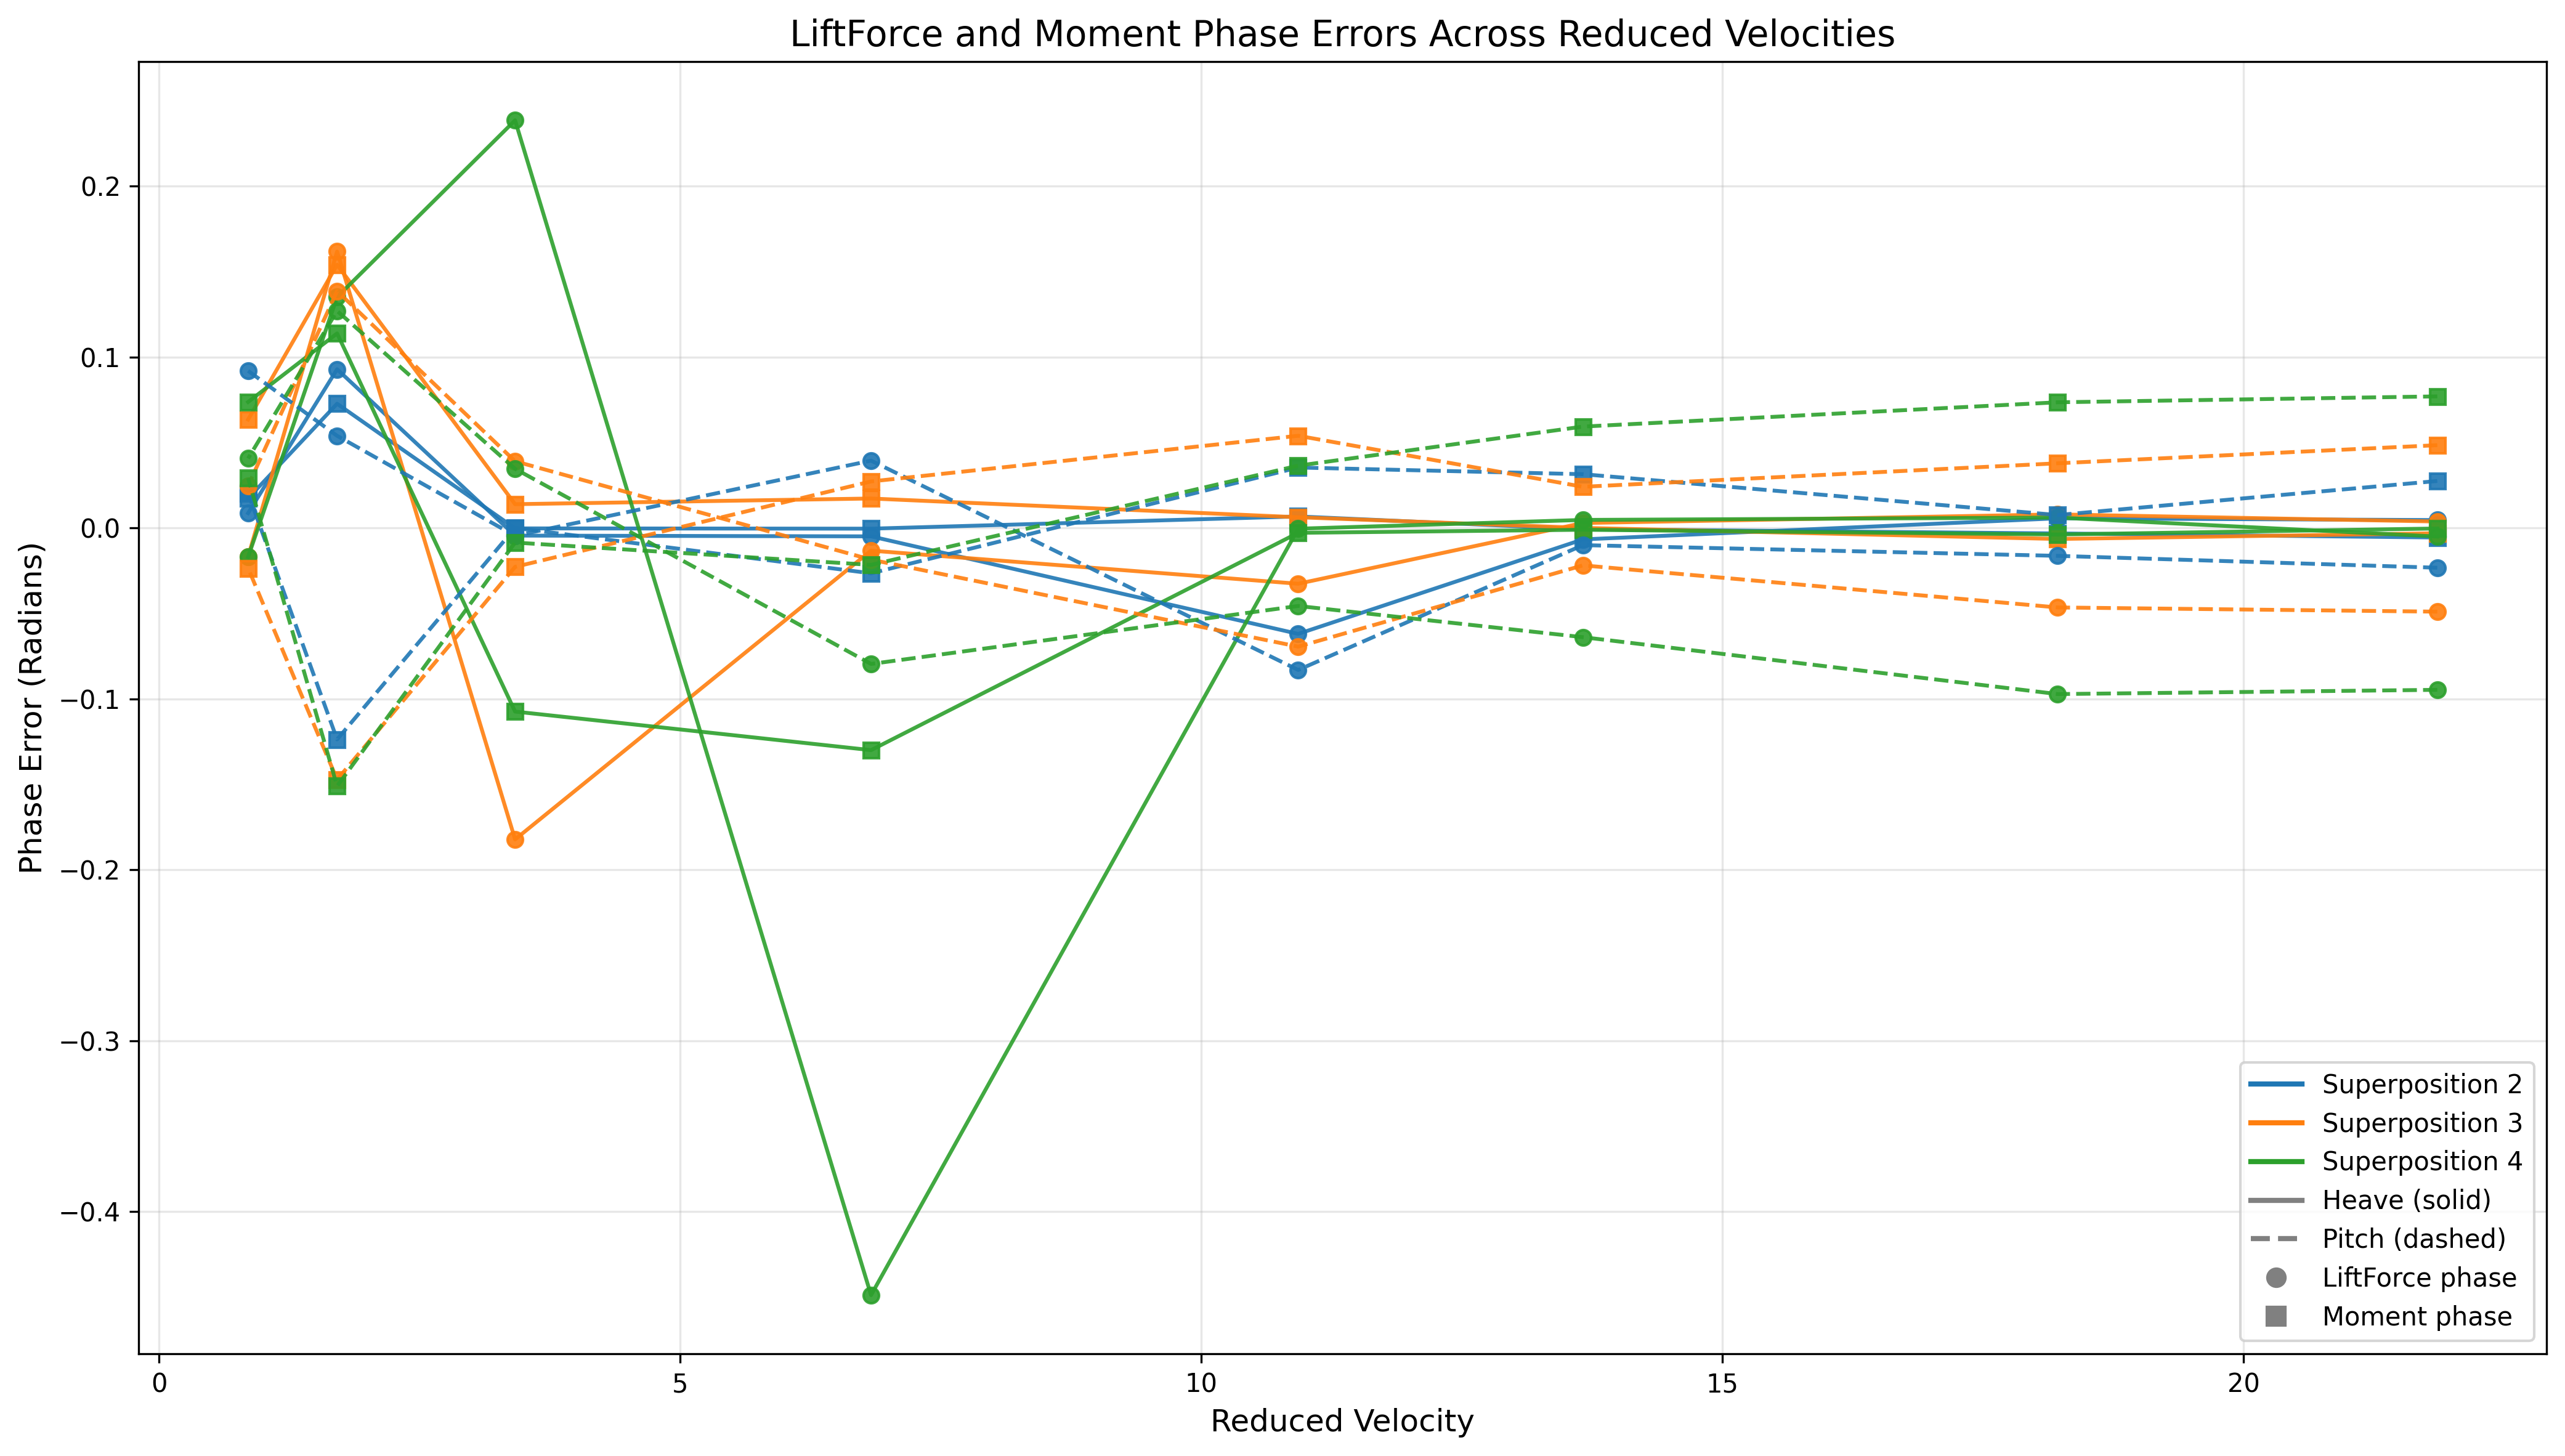
\includegraphics[width=1\textwidth]{Figures/MultiFrequency_Study_1/Combined_Phase_Errors.png}
    \caption{Phase errors as a function of reduced velocity - Campaign~1}
    \label{fig: Phase_Errors}
\end{figure}

The compiled prescribed motion amplitude Vs force plot (Figure~\ref{fig:MF1_Compiled_Displacement_Vs_Force}) 
is analogous to the plot in the nonlinearity study (Figure~\ref{fig:Compiled_Displacement_Vs_Force}). 
From this figure, above the reduced velocity of 6.83, 
the nonlinearity effect is negligible. Below this value, nonlinearity is clearly present.\\

Another point to note is that, although nonlinearity is present at lower reduced velocities, 
no consistent relationship can be established between the number of frequency combinations and the 
resulting error. A tentative inference is that the deviation in nonlinearity is generally largest 
for superposition scheme~4; however, this is not universal, as for certain reduced velocities the 
error in scheme~3 exceeds that in scheme~4.\\

To illustrate this, consider the phase of the aerodynamic moment Figure~\ref{sub@fig:MF1_Compiled_Heave_PhaseMoment_vs_Superpositions}, where the deviation due to 
nonlinearity is high. At the reduced velocity of 3.42, the error for superposition 
scheme~3 is greater than that for scheme~4. But for the phase of the lift force, the 
error in superposition scheme~2 exceeds that of scheme~3 at most reduced velocities.\\

Combining these observations from the amplitude and phase error analyses with the nonlinearity 
study, it can be concluded that the superposition contributes to the source of error at 
lower reduced velocities, while at higher reduced velocities the error is due to the
the inherent nonlinearity of the cross-section.\\

\begin{figure}[htbp]
    \centering

    \begin{subfigure}[b]{0.45\textwidth}
        \centering
        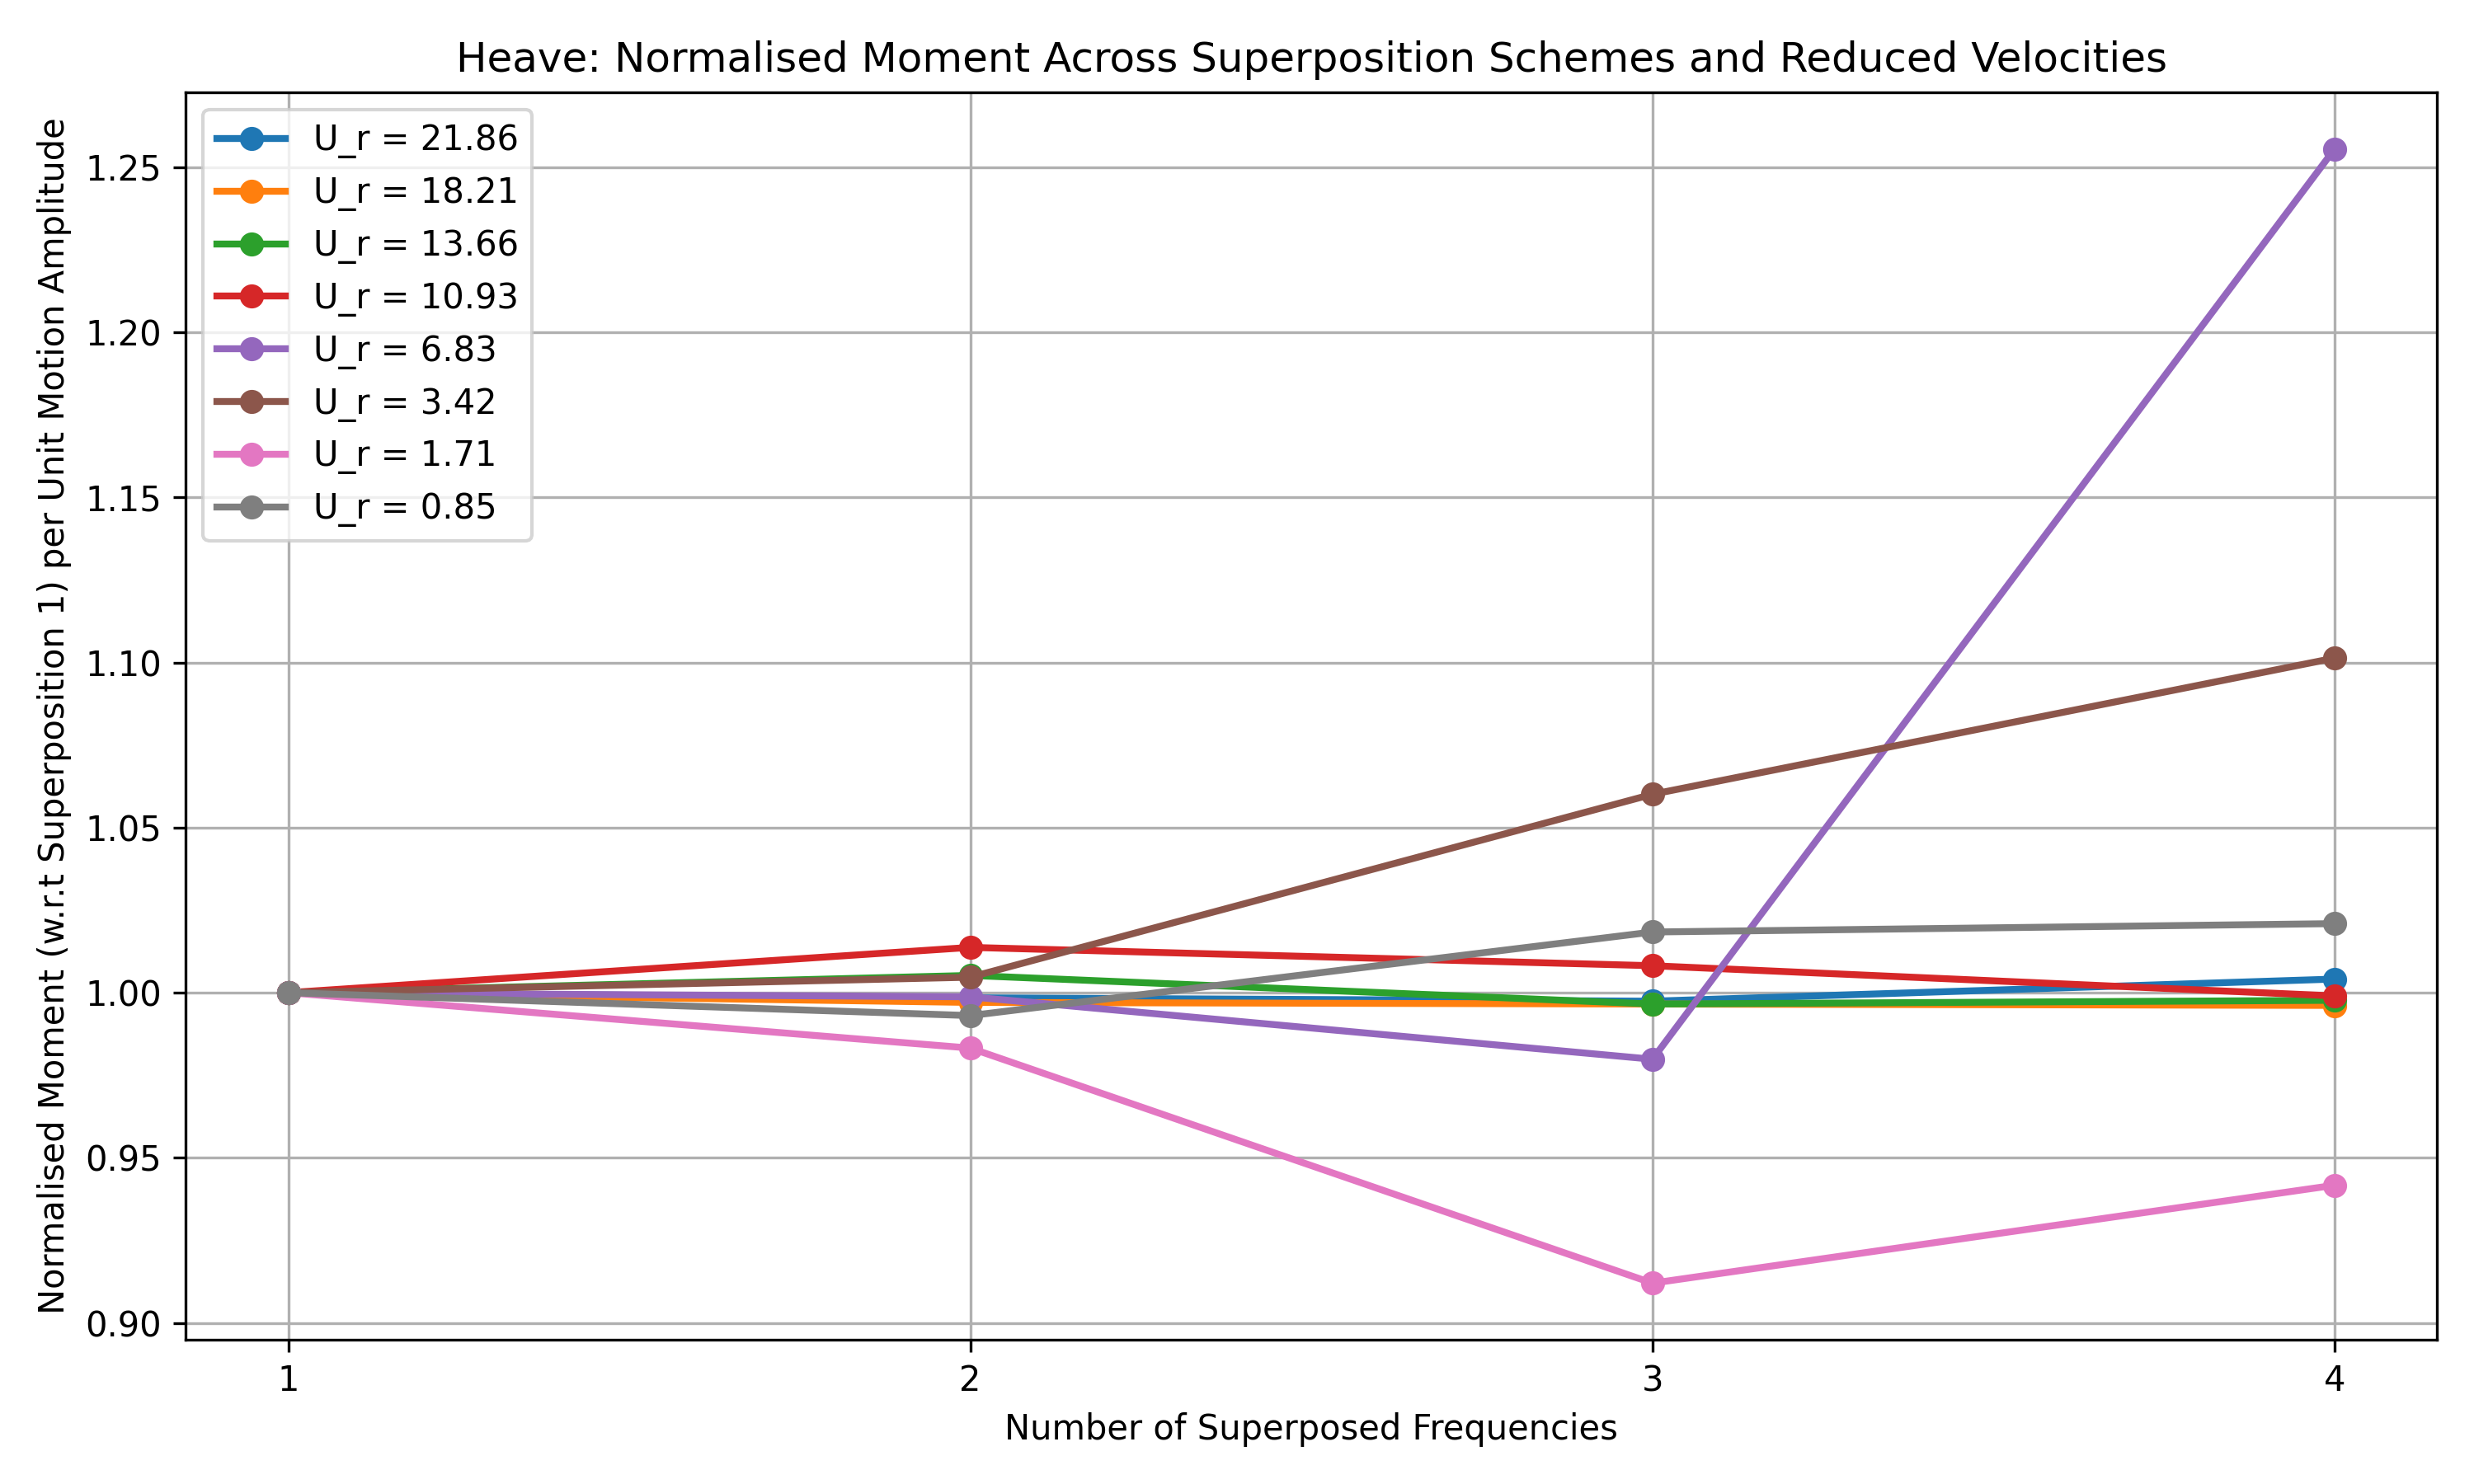
\includegraphics[width=\textwidth]{Figures/MultiFrequency_Study_1/Compressed_Displacement_Vs_Force/Heave/NormalizedMoment_vs_Superpositions_RelativeToFirst.png}
        \caption{}
        \label{fig:MF1_Compiled_Heave_Moment_vs_Superpositions}
    \end{subfigure}
    \hfill
    \begin{subfigure}[b]{0.45\textwidth}
        \centering
        
\includegraphics[width=\textwidth]{Figures/MultiFrequency_Study_1/Compressed_Displacement_Vs_Force/Pitch/NormalizedMoment_vs_Superpositions_RelativeToFirst.png}
        \caption{}
        \label{fig:MF1_Compiled_Pitch_Moment_vs_Superpositions}
    \end{subfigure}

    \begin{subfigure}[b]{0.45\textwidth}
        \centering
        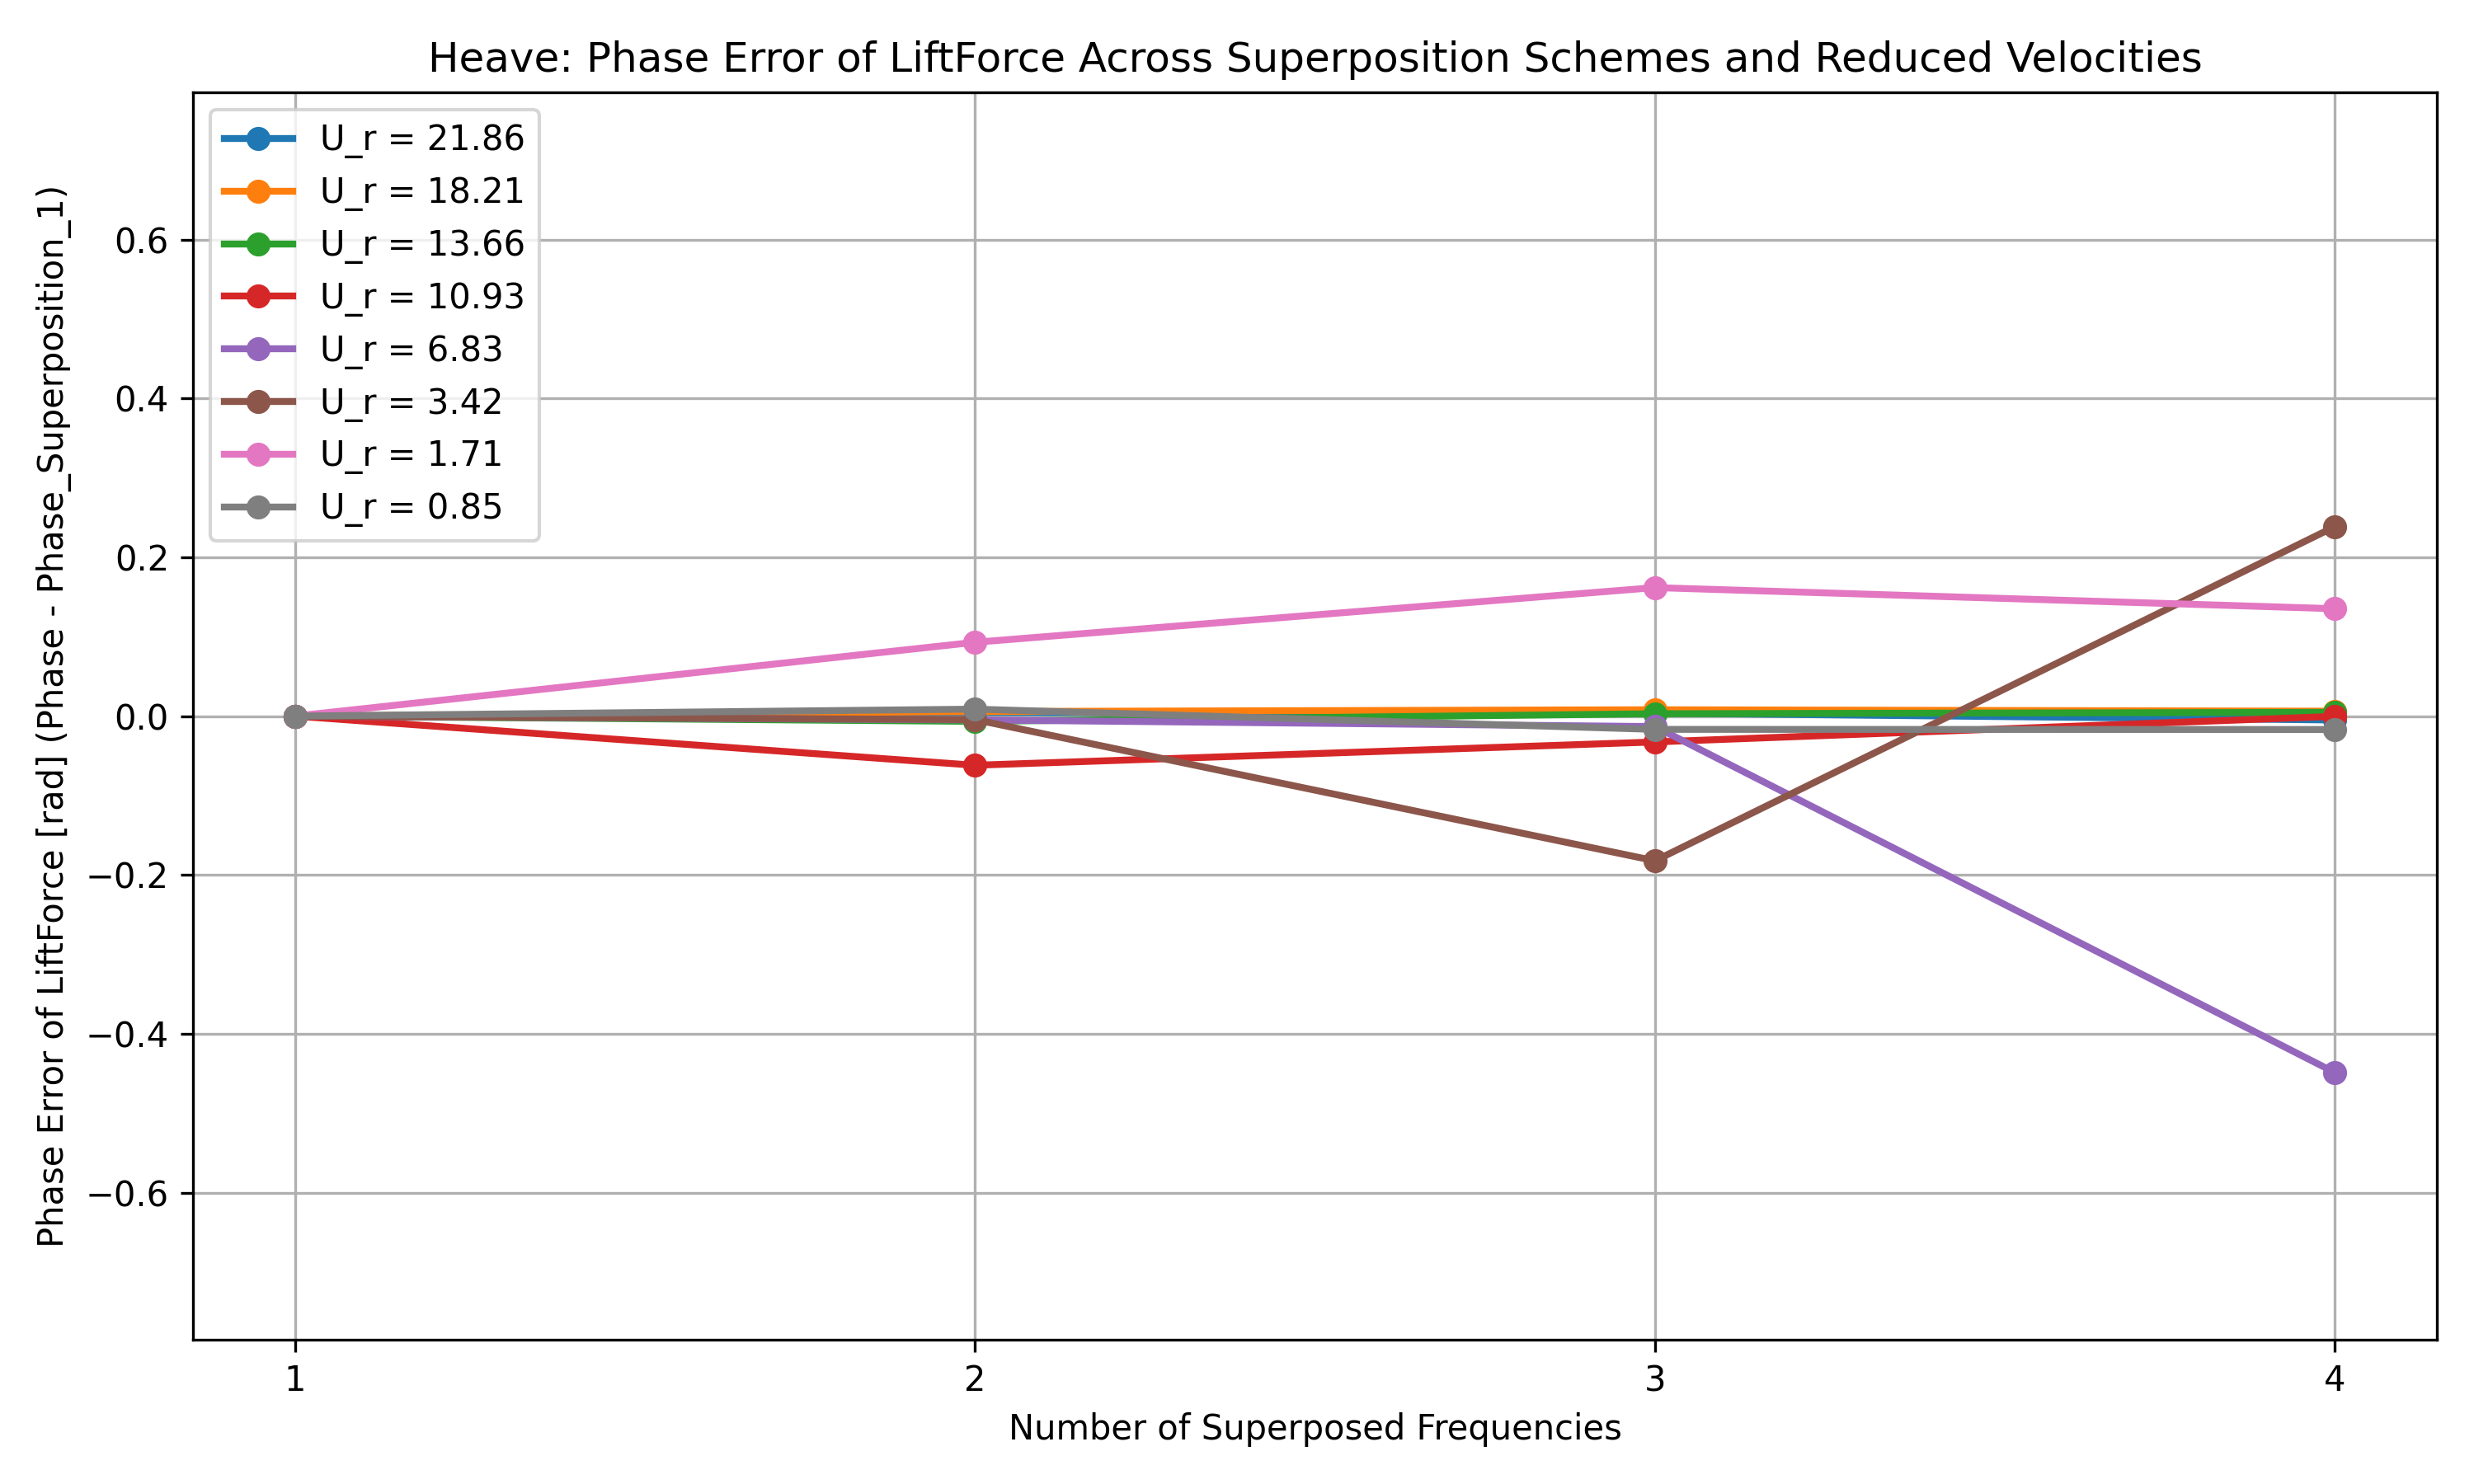
\includegraphics[width=\textwidth]{Figures/MultiFrequency_Study_1/Compressed_Displacement_Vs_Force/Heave/PhaseLiftForce_Error_vs_Superpositions.png}
        \caption{}
        \label{fig:MF1_Compiled_Heave_PhaseLiftForce_Error_vs_Superpositions}
    \end{subfigure}
    \hfill
    \begin{subfigure}[b]{0.45\textwidth}
        \centering
        
\includegraphics[width=\textwidth]{Figures/MultiFrequency_Study_1/Compressed_Displacement_Vs_Force/Pitch/PhaseMoment_Error_vs_Superpositions.png}
        \caption{}
        \label{fig:MF1_Compiled_Pitch_PhaseMoment_Error_vs_Superpositions}
    \end{subfigure}

    \caption{Compiled displacement vs.\ force - Campaign~1}
    \label{fig:MF1_Compiled_Displacement_Vs_Force}
\end{figure}


\subsection{Frequency Domain Analysis of Aerodynamic Forces}
\label{sec:MF1_FreqDomain}

In this section, the frequency domain of the aerodynamic forces are examined. This study helps 
to further classify the source of nonlinearity, specifically, whether it arises from higher-order 
terms induced by large heave and pitch amplitudes, or from the inherent nonlinearity of the 
cross-section even at low amplitude levels.\\

From the figure ~\ref{fig:Frequency_Domain_Analysis_Heave_MF1} and~\ref{fig:Frequency_Domain_Analysis_Pitch_MF1},
the frequency spectra for 4th superposition schemes is clean, showing only the static 
component, the forced-motion response components, and the vortex shedding component. 
This is observed for other 2 superposition schemes as well which shall be verified from the appendix~\ref{fig:app:Frequency_Domain_Analysis_Heave_MF1}.\\
This strengthens the argument from previous sections: provided the total amplitude remains below the 
linearity limit, no higher-order harmonic terms appear in the aerodynamic response.\\

It should also be noted that if the multi-frequency method is adopted for flutter derivative 
identification, the only outputs available for inspection are the flutter derivative plot and 
the frequency domain analysis. The inherent nonlinearity of the cross-section therefore cannot 
be detected from these outputs alone.\\


\begin{figure}[htbp]  
    \centering
    \begin{subfigure}[b]{0.45\textwidth}
        \centering
        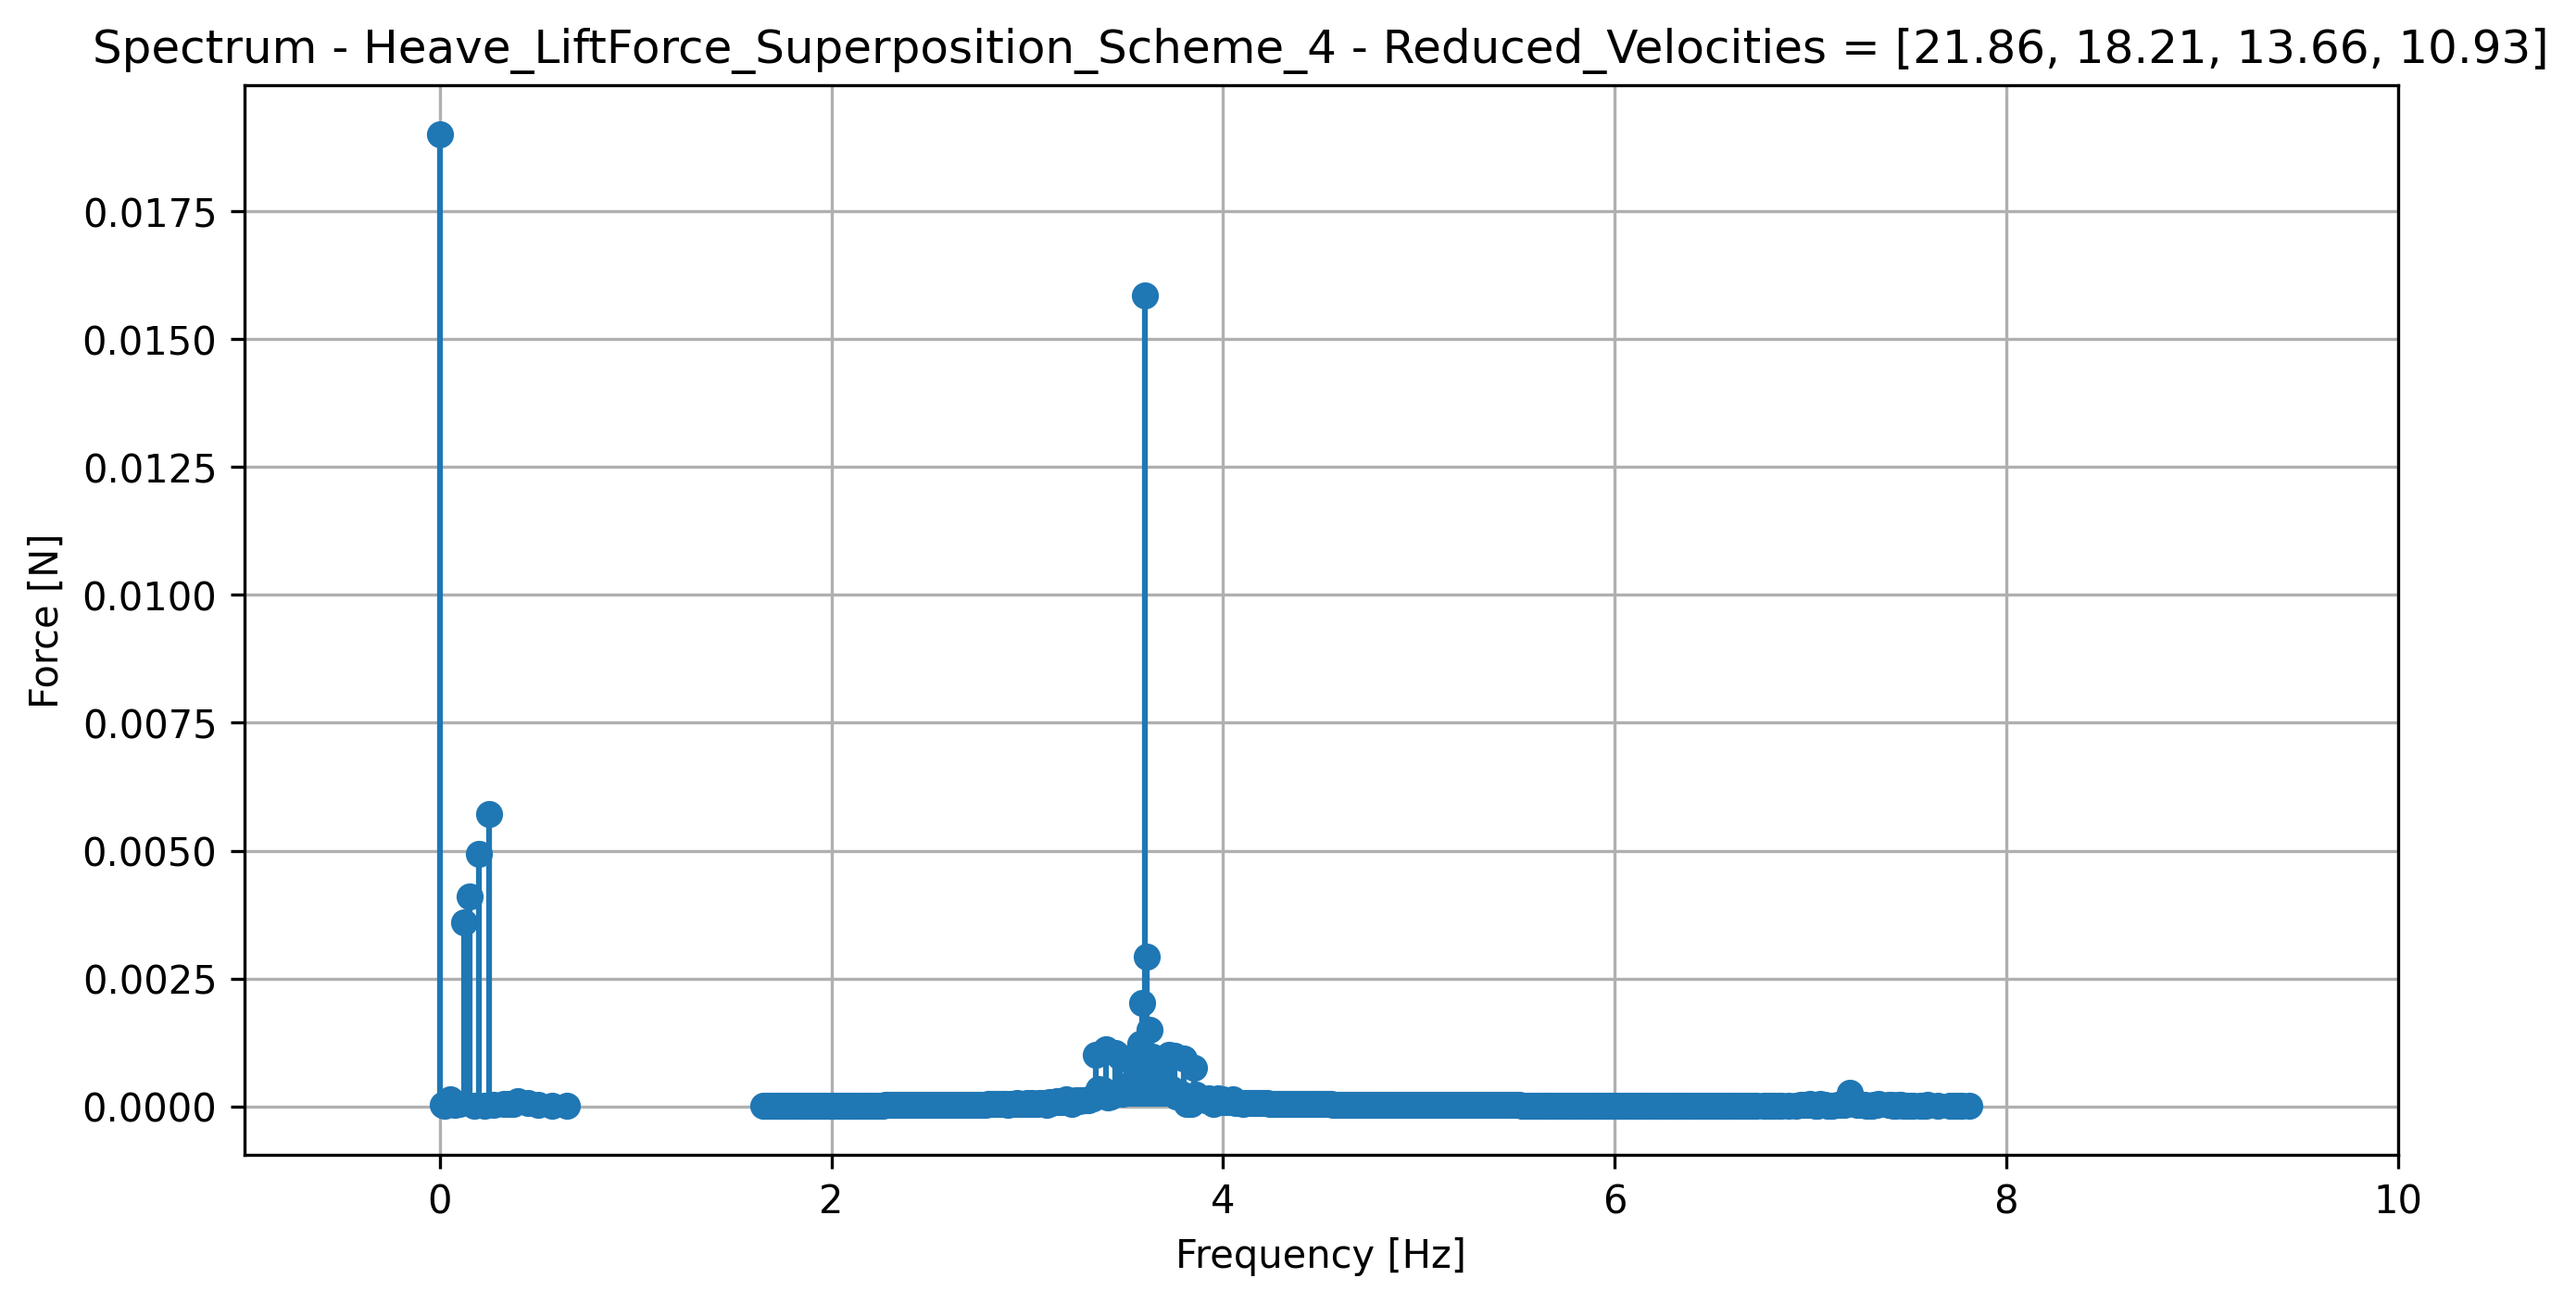
\includegraphics[width=\textwidth]{Figures/MultiFrequency_Study_1/Frequency_Domain_Analysis/Heave/DFT_LiftForce_Superposition_Scheme_4.png}
        \caption{}
        \label{fig:Heave_DFT_Fy_amplitude_case_6}
    \end{subfigure}
    \hfill
    \begin{subfigure}[b]{0.45\textwidth}
        \centering
        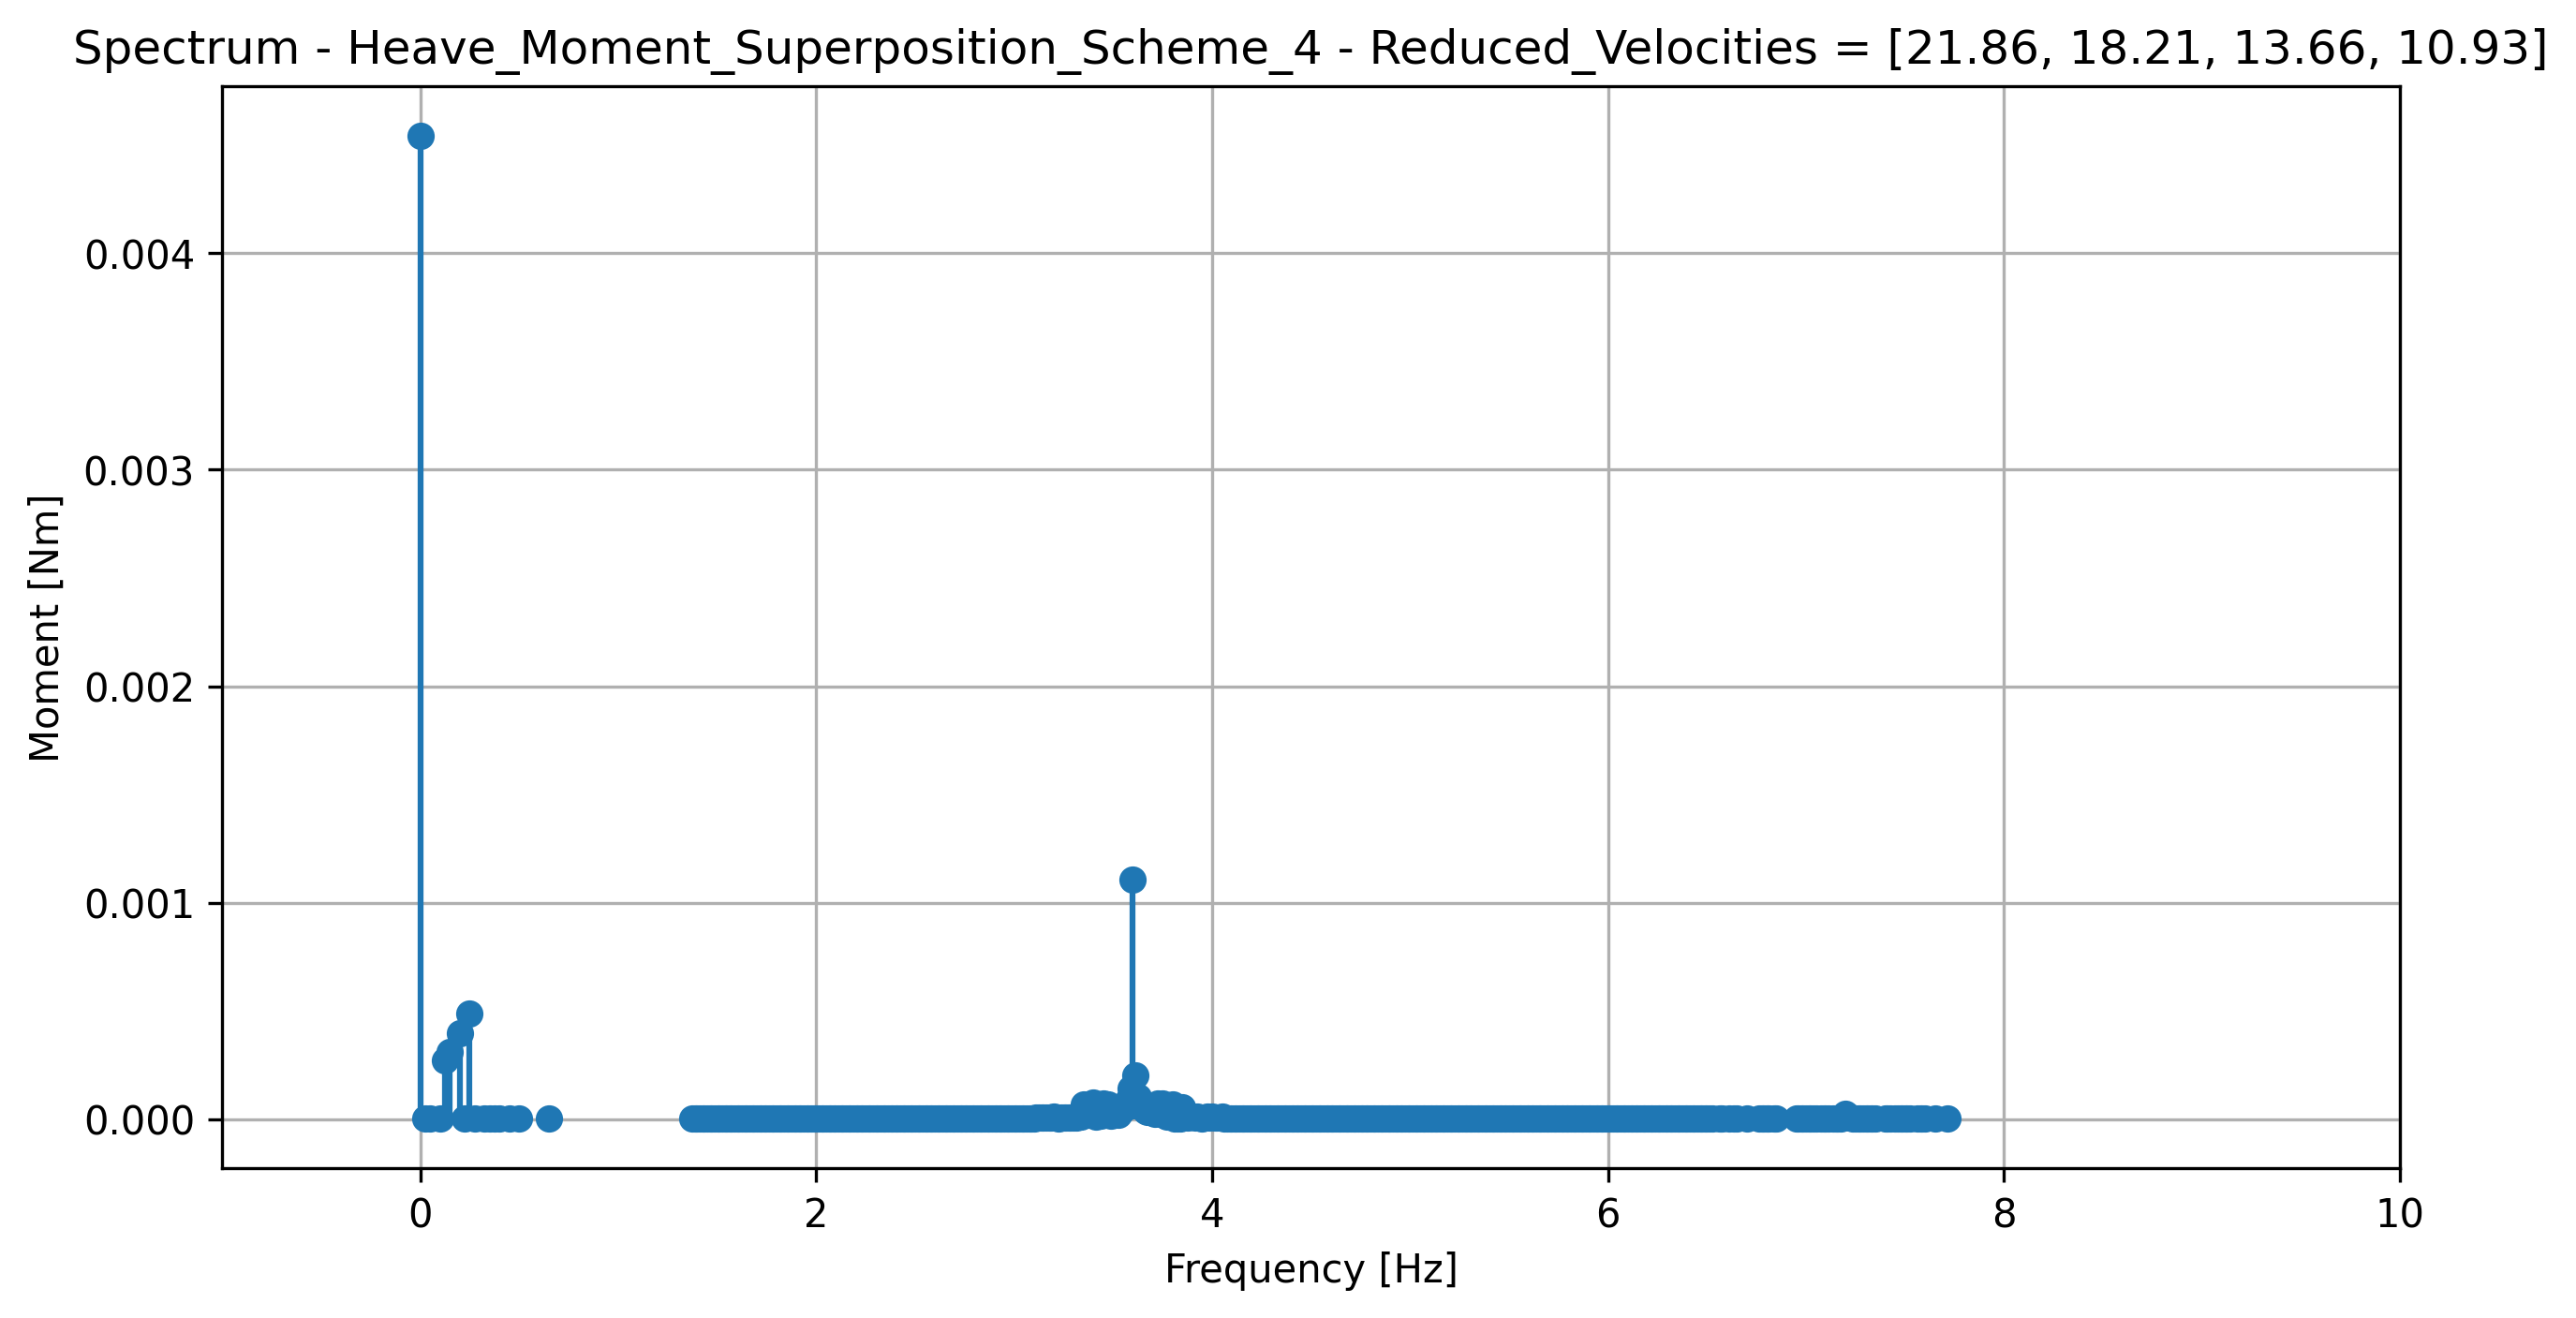
\includegraphics[width=\textwidth]{Figures/MultiFrequency_Study_1/Frequency_Domain_Analysis/Heave/DFT_Moment_Superposition_Scheme_4.png}
        \caption{}
        \label{fig:Heave_DFT_moment_amplitude_case_6}
    \end{subfigure}
    
    \caption{Frequency domain analysis of aerodynamic forces - Heave, Campaign~1}
    \label{fig:Frequency_Domain_Analysis_Heave_MF1}
\end{figure}


\begin{figure}[htbp]  
    \centering
    \begin{subfigure}[b]{0.45\textwidth}
        \centering
        
\includegraphics[width=\textwidth]{Figures/MultiFrequency_Study_1/Frequency_Domain_Analysis/Pitch/DFT_LiftForce_Superposition_Scheme_4.png}
        \caption{}
        \label{fig:Pitch_DFT_Fy_amplitude_case_6_MF1}
    \end{subfigure}
    \hfill
    \begin{subfigure}[b]{0.45\textwidth}
        \centering
        
\includegraphics[width=\textwidth]{Figures/MultiFrequency_Study_1/Frequency_Domain_Analysis/Pitch/DFT_Moment_Superposition_Scheme_4.png}
        \caption{}
        \label{fig:Pitch_DFT_moment_amplitude_case_6_MF1}
    \end{subfigure}
    
    \caption{Frequency domain analysis of aerodynamic forces - Pitch, Campaign~1}
    \label{fig:Frequency_Domain_Analysis_Pitch_MF1}
\end{figure}

Inspection of the frequency domain at lower reduced velocities shows that the ratio between the 
largest and smallest aerodynamic lift force components in a superposition scheme is the reason for 
the error in lower reduced velocities (below 6.83). This ratio is considerably higher when superposing lower reduced 
velocities than superposing reduced velocities (Figure ~\ref{fig:Reduced Velocity Vs Force Amplitudes}). \\

This is further confirmed by another observation. In superposition scheme~3, the aerodynamic forces for reduced velocity 
of 3.42 can be calculated from two simulation groups (Table - \ref{tab:MF1_SP3} MF1-14 and MF1-15). 
On following the same reasoning, the error for 
MF1~15 of scheme~3 (which pairs 3.42 with lower reduced velocities) should be greater than that 
for MF1~14 (which pairs 3.42 with higher reduced velocities). This is indeed the case. For 
the $H_1$ derivative, the error for MF1~14 of superposition scheme~3 is 0.156\%, while 
for MF1~15 the error is 11.913\%.\\

The reason this effect is less significant for pitch motion is that the ratio of 
aerodynamic lift force between the two extreme reduced velocities within a superposition scheme group is  
smaller in pitch than in heave. Numerically, this ratio is 28.32 for the heave lift force and 
3.186 for the pitch lift force. This is the reason that the effect does not significant 
error in the pitch case.\\


\begin{figure}[htbp]
    \centering
    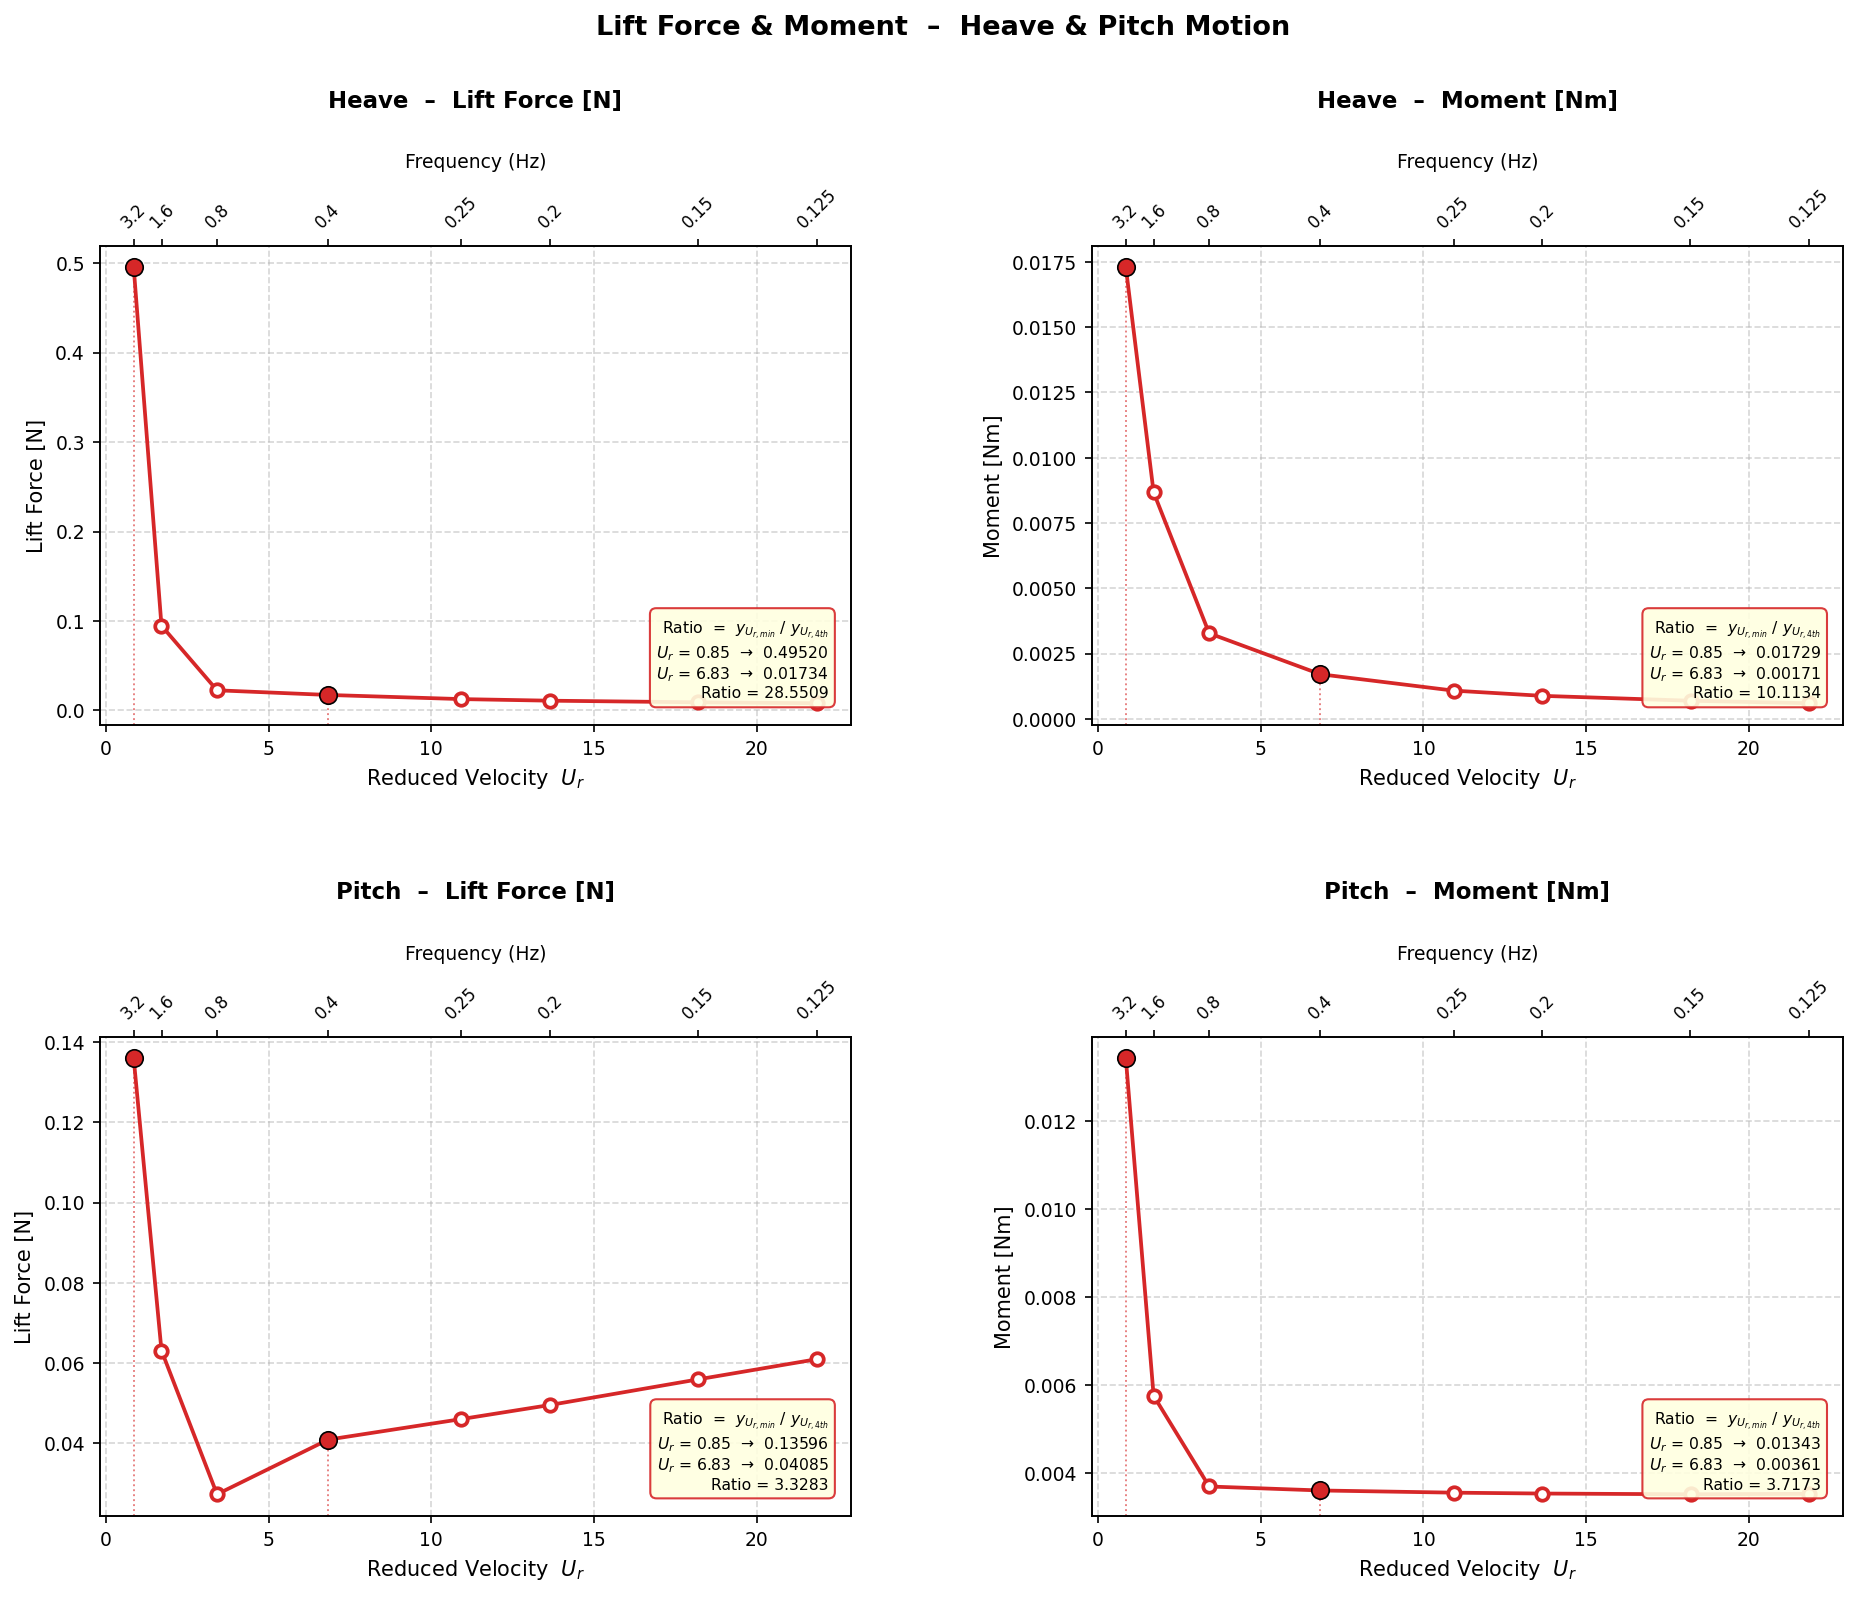
\includegraphics[width=1\textwidth]{Figures/MultiFrequency_Study_1/Heave_Pitch_Amplitude_Plots.png}
    \caption{Reduced Velocity Vs Force Amplitudes}
    \label{fig:Reduced Velocity Vs Force Amplitudes}
\end{figure}


\subsection{Effect on Critical Wind Speed}

% ── MF1 § Effect on Critical Wind Speed ──────────────────────────────────────
Similar to the nonlinearity study on critical velocity, the influence of superposition
schemes on the critical flutter velocity is examined here.
For the bridge structural properties, refer to Table~\ref{tab:bridge_configs}.\\

From Figure~\ref{fig:CriticalVelocity_Vs_Number_of_Superpositions_MF1}, it can be seen that
the critical velocity remains constant for the first three superposition schemes.
For the fourth scheme, a considerable variation is observed, particularly for the Humen Bridge.\\

The reason for this behaviour can be understood by examining the reduced critical velocity
plot (Figure~\ref{fig:ReducedVelocity_Vs_Number_of_Superpositions_MF1}).
It can be observed that for the Humen Bridge, the reduced critical velocity falls below 7.
As discussed earlier, errors in superposition scheme~4 are highest in this lower reduced
velocity range, and these errors are directly reflected in the predicted critical velocity.\\

\begin{figure}[htbp]
    \centering
    \begin{minipage}{0.48\textwidth}
        \centering
        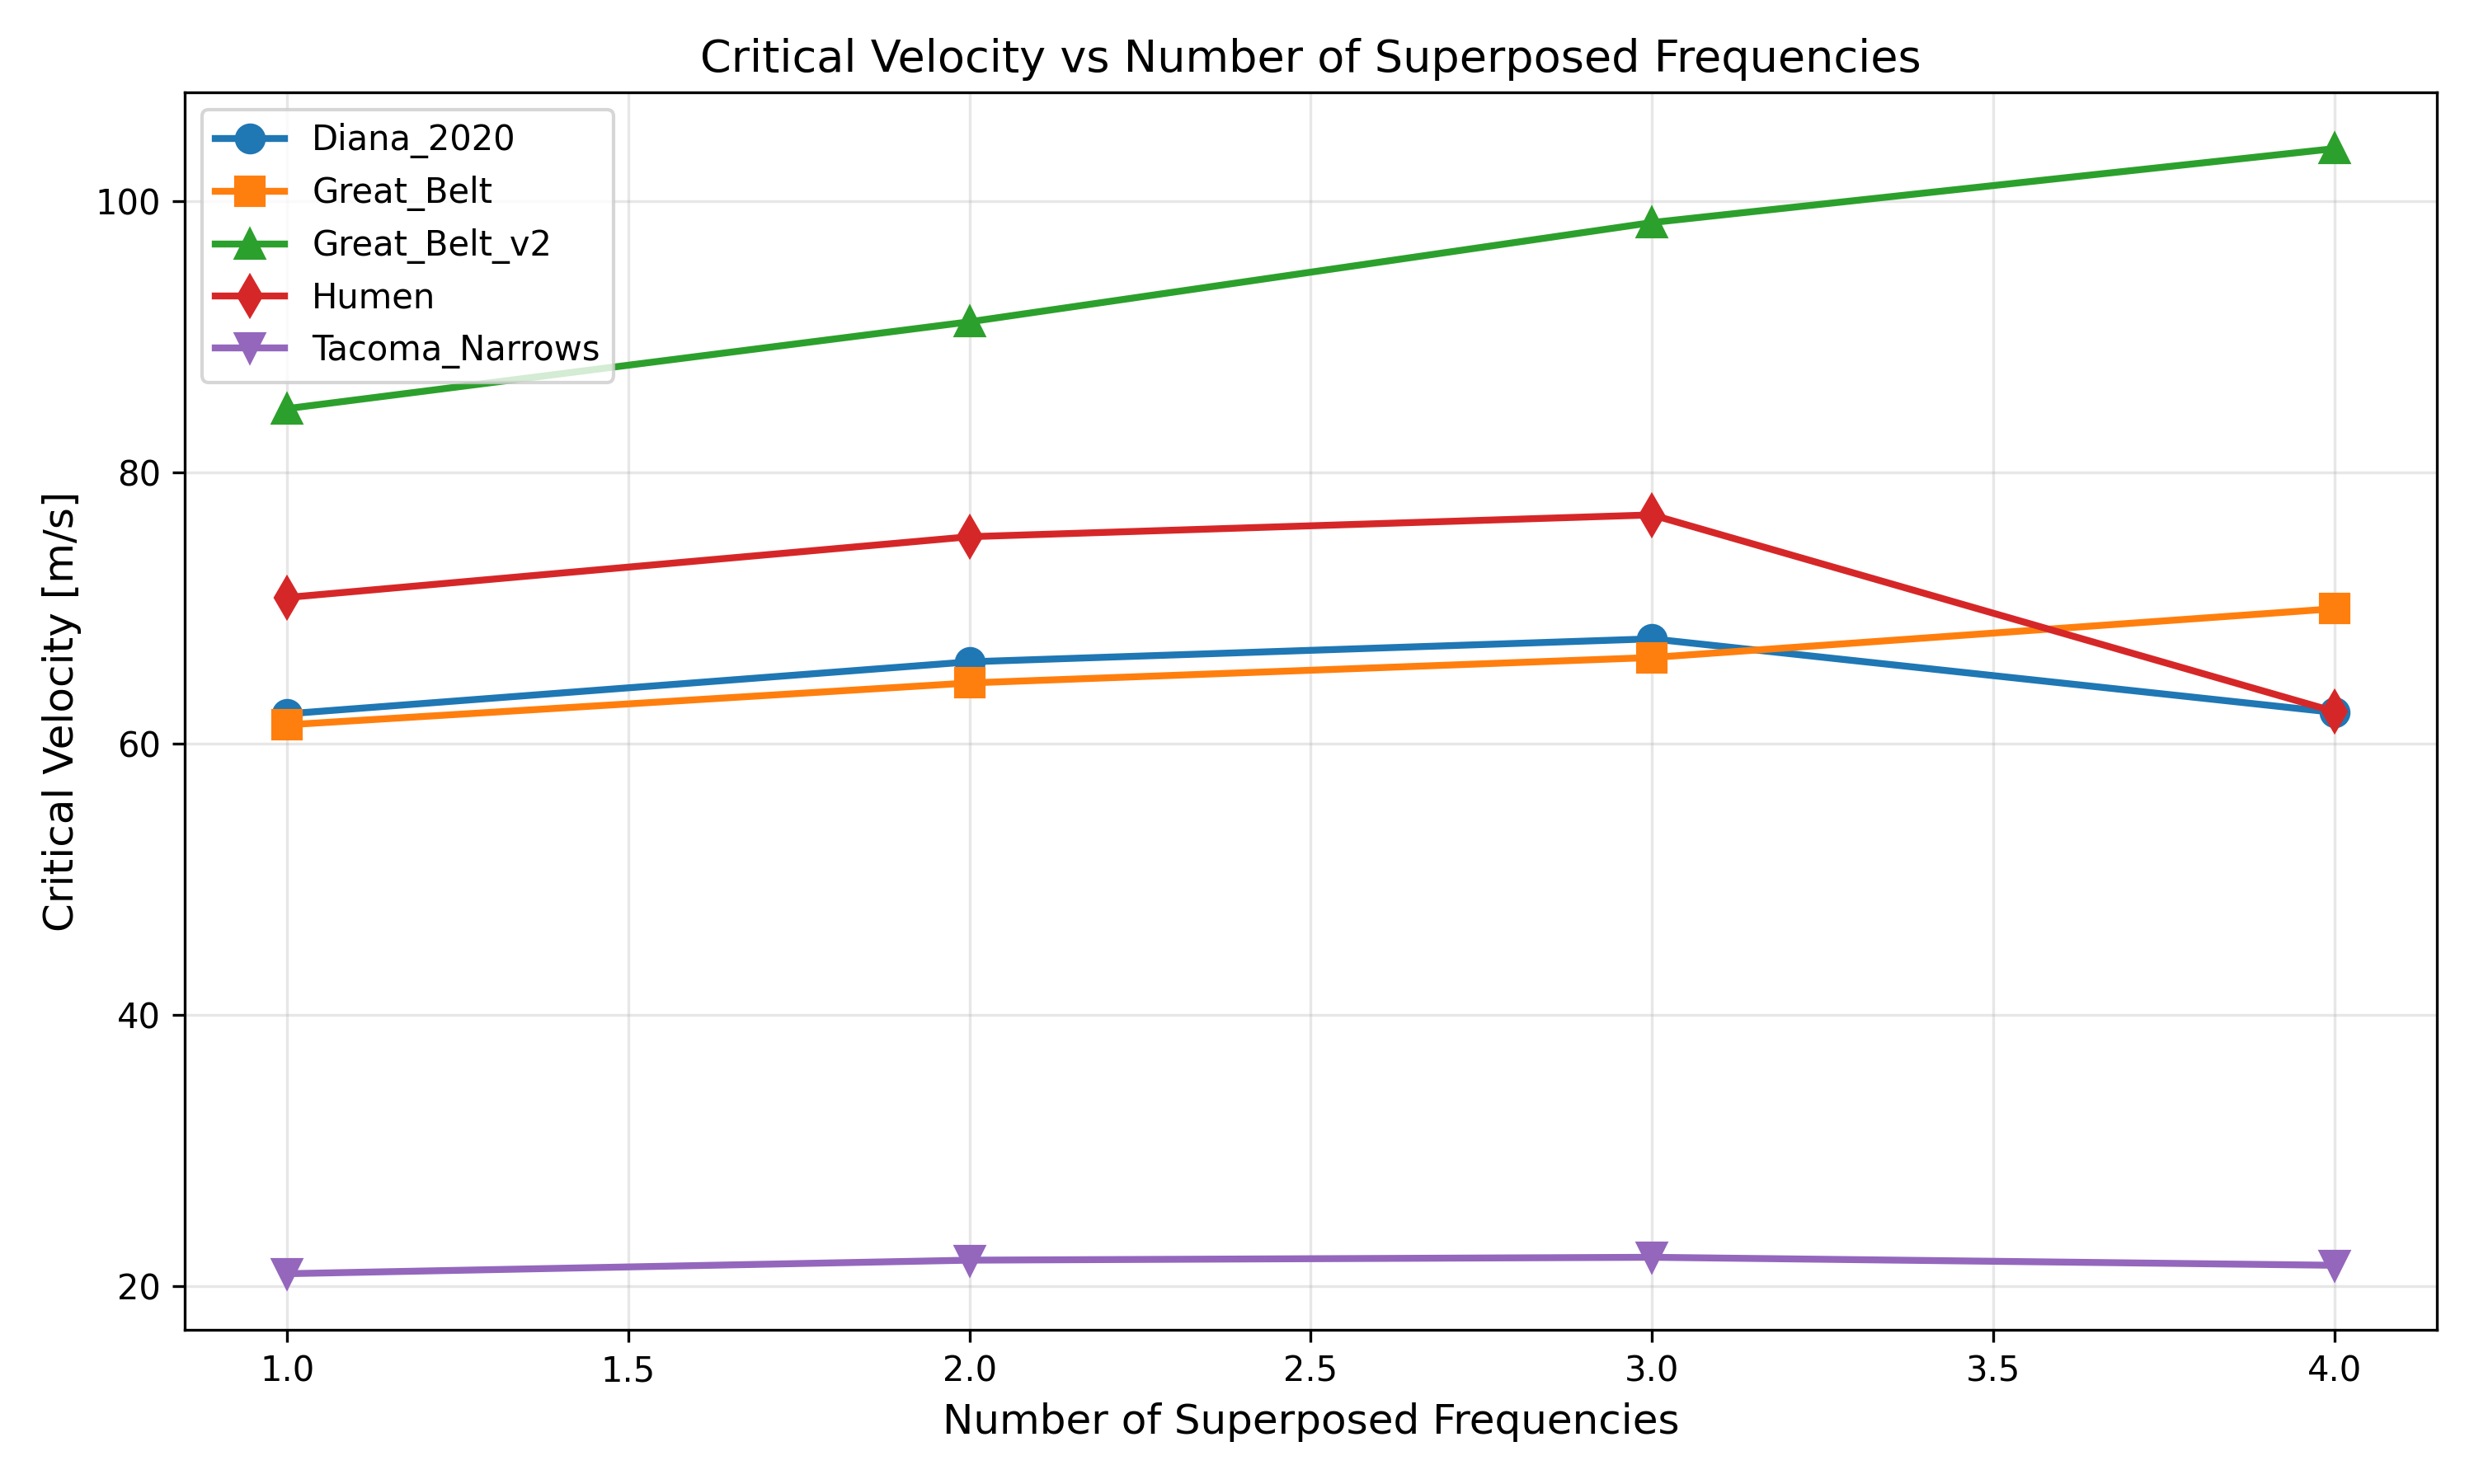
\includegraphics[width=\textwidth]{Figures/MultiFrequency_Study_1/CriticalVelocity_vs_Number_of_Superpositions.png}
        \caption{Critical wind speed vs.\ number of superpositions - Campaign~1}
        \label{fig:CriticalVelocity_Vs_Number_of_Superpositions_MF1}
    \end{minipage}
    \hfill
    \begin{minipage}{0.48\textwidth}
        \centering
        \includegraphics[width=\textwidth]{Figures/MultiFrequency_Study_1/ReducedVelocity_vs_Number_of_Superpositions.png}
        \caption{Reduced critical wind speed vs.\ number of superpositions - Campaign~1}
        \label{fig:ReducedVelocity_Vs_Number_of_Superpositions_MF1}
    \end{minipage}
\end{figure}

% ============================================================
\section{Multi-Frequency Analysis 2}
% ============================================================

In this section, the multi-frequency method is applied with keeping individual precribed motion
amplitudes below the linearity limit obtained from the nonlinearity study.

This section is organised as follows:

\begin{flushleft}
\hspace{2cm}1. Superposition Schemes \\
\hspace{2cm}2. Flutter Derivatives Results and Comparison \\
\hspace{2cm}3. Frequency Domain Analysis of Aerodynamic Forces \\
\hspace{2cm}4. Error Analysis of Aerodynamic Forces \\
\hspace{2cm}5. Effect on Critical Wind Speed \\
\end{flushleft}

\subsection{Superposition Schemes}

Since all prescribed motion amplitude are identical, they are shown in a single table
(Table~\ref{tab:MF2_Params}). The frequency combinations can be mapped using the
superposition scheme defined in Section~\ref{sec:Selection of Frequencies and Superpositions}.\\

\begin{table}[htbp]
\centering
\caption{Frequencies and Amplitude Parameters for Multi-Frequency Campaign~2}
\label{tab:MF2_Params}
\begin{tabular}{|l|cccccccc|}
\hline
\rule{0pt}{12pt}\textbf{Frequency (Hz)} & 0.125 & 0.15 & 0.2 & 0.25 & 0.4 & 0.8 & 1.6 & 3.2 \\[4pt]
\hline
Reduced Velocity        & 21.86 & 18.21 & 13.66 & 10.93 & 6.83 & 3.42 & 1.71 & 0.85 \\
Stable Time Period (s)  & 80    & 80    & 50    & 40    & 25   & 12.5 & 6.25 & 3.125 \\
Heave Amplitude (m)     & 0.0183 & 0.0183 & 0.0183 & 0.0183 & 0.0183 & 0.0183 & 0.0183 & 0.0183 \\
Pitch Amplitude (rad)   & 0.087 & 0.087 & 0.087 & 0.087 & 0.087 & 0.087 & 0.087 & 0.087 \\
\hline
\end{tabular}
\end{table}

\subsection{Flutter Derivatives Results and Comparison}

\begin{figure}[htbp]
    \centering
    
\includegraphics[width=1\textwidth]{Figures/MultiFrequency_Study_2/Combined_Flutter_Derivative.png}
    \caption{Flutter derivatives - Campaign~2}
    \label{fig:Combined_Flutter_Derivatives_2}
\end{figure}

From the Figure~\ref{fig:Combined_Flutter_Derivatives_2}, it can be observed, the flutter derivatives exhibit
significant variation across superposition schemes, particularly for $H_2$ and $A_2$.
A notable variation is also present in $H_4$ and $A_4$, whereas $H_1$ and $A_1$ show
comparatively little variation. The key observation here is that the keeping individual amplitude below the nonlinearity threshold 
produces large errors. Hence sum of the amplitudes
across all frequencies in a superposition scheme group must be kept below the nonlinearity threshold,
as shown in the previous campaign.\\

\subsection{Error Analysis of Aerodynamic Forces}

From the error analysis (Figure~\ref{fig:Amplitude_Errors_MF2}), the errors in the aerodynamic
lift force and moment for pitch motion average approximately 20\%, while for heave motion they
are around 10\%. The phase errors for pitch motion are approximately 0.2~radians, which is
because of inherent nonlinearity of the cross-section.\\

\begin{figure}[htbp]
    \centering
    
\includegraphics[width=1\textwidth]{Figures/MultiFrequency_Study_2/Combined_Amplitude_Errors.png}
    \caption{Amplitude errors as a function of reduced velocity - Campaign~2}
    \label{fig:Amplitude_Errors_MF2}
\end{figure}

\begin{figure}[htbp]
    \centering
    
\includegraphics[width=1\textwidth]{Figures/MultiFrequency_Study_2/Combined_Phase_Errors.png}
    \caption{Phase errors as a function of reduced velocity - Campaign~2}
    \label{fig:Phase_Errors_MF2}
\end{figure}

\subsection{Frequency Domain Analysis of Aerodynamic Forces}

From the frequency domain analysis for heave motion
(Figure~\ref{fig:Frequency_Domain_Analysis_Heave_MF2}), higher-order harmonic terms begin to
appear as the number of superposed frequencies increases, although they are not very significant. 
These higher-order terms are the primary cause of the significant variation
errors in the $H_4$ and $A_4$ derivatives.\\

\begin{figure}[htbp]  
    \centering   
    \begin{subfigure}[b]{0.45\textwidth}
        \centering
        
\includegraphics[width=\textwidth]{Figures/MultiFrequency_Study_2/Frequency_Domain_Analysis/Heave/DFT_LiftForce_Superposition_Scheme_4.png}
        \caption{}
        \label{fig:Heave_DFT_Fy_amplitude_case_6_MF2}
    \end{subfigure}
    \hfill
    \begin{subfigure}[b]{0.45\textwidth}
        \centering
        
\includegraphics[width=\textwidth]{Figures/MultiFrequency_Study_2/Frequency_Domain_Analysis/Heave/DFT_Moment_Superposition_Scheme_4.png}
        \caption{}
        \label{fig:Heave_DFT_moment_amplitude_case_6_MF2}
    \end{subfigure}
    
    \caption{Frequency domain analysis of aerodynamic forces - Heave, Campaign~2}
    \label{fig:Frequency_Domain_Analysis_Heave_MF2}
\end{figure}

On examining the frequency domain for pitch motion
(Figure~\ref{fig:Frequency_Domain_Analysis_Pitch_MF2}), the spectrum becomes increasingly
noisy as the number of superposed frequencies increases. This spectral leakage is the
primary reason for the large errors observed in the $H_2$ and $A_2$ derivatives.
An important conclusion from this section is that the frequency domain analysis is a
reliable tool for nonlinearity identification. It can clearly identify nonlinearity arising from a violation of
the scanlan's linearity assumption.\\ 

\begin{figure}[htbp]  
    \centering 
    \begin{subfigure}[b]{0.45\textwidth}
        \centering
        
\includegraphics[width=\textwidth]{Figures/MultiFrequency_Study_2/Frequency_Domain_Analysis/Pitch/DFT_LiftForce_Superposition_Scheme_4.png}
        \caption{}
        \label{fig:Pitch_DFT_Fy_amplitude_case_6_MF2}
    \end{subfigure}
    \hfill
    \begin{subfigure}[b]{0.45\textwidth}
        \centering
        
\includegraphics[width=\textwidth]{Figures/MultiFrequency_Study_2/Frequency_Domain_Analysis/Pitch/DFT_Moment_Superposition_Scheme_4.png}
        \caption{}
        \label{fig:Pitch_DFT_moment_amplitude_case_6_MF2}
    \end{subfigure}
    
    \caption{Frequency domain analysis of aerodynamic forces - Pitch, Campaign~2}
    \label{fig:Frequency_Domain_Analysis_Pitch_MF2}
\end{figure}

\subsection{Effect on Critical Wind Speed}

The influence of superposition on the critical flutter velocity is expected to be high
in this campaign, as the errors are large in the flutter derivatives. The critical velocities
show significant variation across superposition schemes, as seen in
Figures~\ref{fig:CriticalVelocity_Vs_Number_of_Superpositions_MF2}
and~\ref{fig:ReducedVelocity_Vs_Number_of_Superpositions_MF2}.
However, the variations are not as severe for the Great Belt Bridge and the DIANA reference
configuration, which indicates that the influence of the $H_2$ and $A_2$ derivative on the critical
wind speed is relatively minor for these two configurations.\\

\begin{figure}[htbp]
    \centering
    \begin{minipage}{0.48\textwidth}
        \centering
        
\includegraphics[width=\textwidth]{Figures/MultiFrequency_Study_2/CriticalVelocity_vs_Number_of_Superpositions.png}
        \caption{Critical wind speed vs.\ number of superpositions - Campaign~2}
        \label{fig:CriticalVelocity_Vs_Number_of_Superpositions_MF2}
    \end{minipage}
    \hfill
    \begin{minipage}{0.48\textwidth}
        \centering
        \includegraphics[width=\textwidth]{Figures/MultiFrequency_Study_2/ReducedVelocity_vs_Number_of_Superpositions.png}
        \caption{Reduced critical wind speed vs.\ number of superpositions - Campaign~2}
        \label{fig:ReducedVelocity_Vs_Number_of_Superpositions_MF2}
    \end{minipage}
\end{figure}

% ------------------------------------------------------------
\section{Key Findings}
% ------------------------------------------------------------

The multi-frequency forced-motion CFD simulations reveal distinct patterns in the accuracy of flutter derivative identification. 
Flutter derivatives $H_1$, $H_3$, $A_1$, and $A_3$ are accurately identified across all superposition schemes. In contrast, 
flutter derivatives $H_2$, $H_4$, $A_2$, and $A_4$ exhibit notable errors in the multi-frequency forced-motion CFD simulation. 
These discrepancies arise from the frequency-domain response under pitch excitation, which contains higher-order harmonic terms 
indicating the presence of nonlinearity. This nonlinearity specifically affects the pitch-motion-associated derivatives: $H_2$, 
$H_3$, $A_2$, and $A_3$. Importantly, these errors in flutter derivative identification have a significant influence on the 
predicted critical flutter velocity, which must be carefully considered when applying the multi-frequency method for bridge 
design and safety analysis.

\begin{figure}[htbp]
    \centering
    
\includegraphics[width=0.75\textwidth]{Figures/Simulation_Time.png}
    \caption{Simulation time}
    \label{fig:Simulation_Time}
\end{figure}

% ============================================================
\section{Framework for Multi-Frequency Analysis}
% ============================================================

Based on the results obtained above, the following framework is proposed for conducting a 
multi-frequency analysis.

\begin{enumerate}
    \item \textbf{Determine the number of superpositions.} The recommended number is 3 or 4.

    \item \textbf{Target the lower frequency range.} Superpositions should preferably be formed 
          from the lowest frequencies (i.e.\ those at the highest reduced velocities).

    \item \textbf{Select one independent frequency per superposition.}

    \item \textbf{Derive the dependent frequencies} within each superposition such that they 
          fall within the frequency bin of the independent frequency. A detailed procedure 
          for this calculation is shown at the start of this chapter.

    \item \textbf{Select amplitudes} such that the total amplitude (sum across all frequencies 
          in a superposition) remains below a heave ratio of 5\% and a pitch angle of 3°.

    \item \textbf{Post-processing:} Apply the Discrete Fourier Transform (DFT) to the 
          aerodynamic forces and moments to extract individual frequency components. 
          The spectrum should also be inspected for signs of nonlinearity.
\end{enumerate}

\vspace{0.5em}
\textbf{Important Notes:}

Accurate application of the discrete Fourier transform (DFT) requires careful consideration of frequency bin placement. 
Because DFT is used, accurate spectral decomposition of the aerodynamic forces is only achievable for frequency components 

that fall exactly within a frequency bin, and accurate results cannot be obtained for frequencies that fall between bins. 
Moreover, even if a frequency of interest falls exactly within a frequency bin, spectral leakage from a neighbouring frequency 
that does \emph{not} fall within a bin can contaminate the extracted amplitude and phase at that frequency. Therefore, when 
selecting frequencies, it is essential to avoid choosing two that are consecutive in the frequency bin list, as sufficient 
spacing between selected frequencies significantly reduces the impact of spectral leakage and ensures reliable flutter 
derivative extraction.

\vspace{0.5em}
% \textbf{Selection of Dependent Frequencies:}


\end{document}